% Panel B explained, T3 in full, and the figure for T3.
% 2026-09-16. Companion to output/2026-09-16_table1-dossier/.
\documentclass[10pt,a4paper]{article}

\usepackage[T1]{fontenc}
\usepackage[utf8]{inputenc}
\usepackage[margin=2.1cm,bottom=2.4cm]{geometry}
\usepackage{pdflscape}
\usepackage{longtable}
\usepackage{booktabs}
\usepackage{array}
\usepackage{amsmath,amssymb}
\usepackage{graphicx}
\usepackage{xcolor}
\usepackage{caption}
\usepackage{quoting}
\usepackage[hidelinks]{hyperref}
\usepackage{titlesec}
\usepackage{fancyhdr}
\usepackage{tcolorbox}
\tcbuselibrary{skins,breakable}

\captionsetup{font=small,labelfont=bf,skip=5pt}
\renewcommand{\arraystretch}{1.1}
\setlength{\tabcolsep}{4pt}
\quotingsetup{leftmargin=1.4em,rightmargin=1.4em,vskip=5pt}

\definecolor{rule}{HTML}{8A8A94}
\definecolor{soft}{HTML}{F4F4F6}
\newtcolorbox{verdict}[1][]{colback=soft,colframe=rule,boxrule=0.4pt,
  left=6pt,right=6pt,top=5pt,bottom=5pt,breakable,#1}

\titleformat{\section}{\large\bfseries}{\thesection}{0.6em}{}
\titleformat{\subsection}{\normalsize\bfseries}{\thesubsection}{0.6em}{}
\titleformat{\subsubsection}[runin]{\normalsize\bfseries}{}{0pt}{}[.]

\pagestyle{fancy}
\fancyhf{}
\fancyhead[L]{\footnotesize Panel B, T3, and the figure}
\fancyhead[R]{\footnotesize 2026-09-16}
\fancyfoot[C]{\footnotesize\thepage}
\renewcommand{\headrulewidth}{0.3pt}

\begin{document}

\begin{center}
{\LARGE\bfseries What Panel B measures, T3 in full,}\\[2pt]
{\LARGE\bfseries and the figure that should carry it}\\[8pt]
{\normalsize José Lucas de Melo Costa \quad$\cdot$\quad 16 September 2026}\\[4pt]
{\footnotesize Companion to the Table 1 dossier. Every number is read from the stored results at
build time; the script that draws the figures reproduces all 27 published cells of the source table.}
\end{center}
\vspace{4pt}
\hrule
\vspace{10pt}

\section{What the numbers in Panel B are}

Every cell holds two numbers separated by a slash. The second one is easy: it is the raw coverage,
the fraction of problems on which the interval the procedure actually reported contained the true
causal effect. The first one is the whole design of the table, and it is not a width in effect units.
It is the answer to this question:

\begin{quoting}
\emph{If we forced this procedure to be honest, how wide would it have to be, compared with the
width that throwing the knowledge away would need?}
\end{quoting}

The reason the table is built that way is that a raw width and a raw coverage, printed as two free
columns, let any procedure shelter in one of them. Discarding the knowledge and reporting the
interval over every graph the data allows covers the truth essentially always, in every regime. It
passes any coverage gate that could be written. So the argument has to happen in the width column,
and a width column is only meaningful between procedures that cover equally. Calibrating first, then
measuring width, is what makes the comparison fair.

\subsection{Step 1. How far off is one reported interval}

Take a single problem at a single sample: a network, a treatment, an outcome, one random draw of
data. The procedure reports an interval. It has a midpoint and a half-width. The true effect is
known, because the data was generated from a graph we hold.

Measure the distance from the interval's midpoint to the truth, in units of the interval's own
half-width. Call it $\lambda_i$. A value below one means the interval already contains the truth.
A value of exactly one means it reaches it at the endpoint. A value of three means the interval
would have to be made three times wider, about its own midpoint, before it touched the truth.

\begin{figure}[h]
\centering
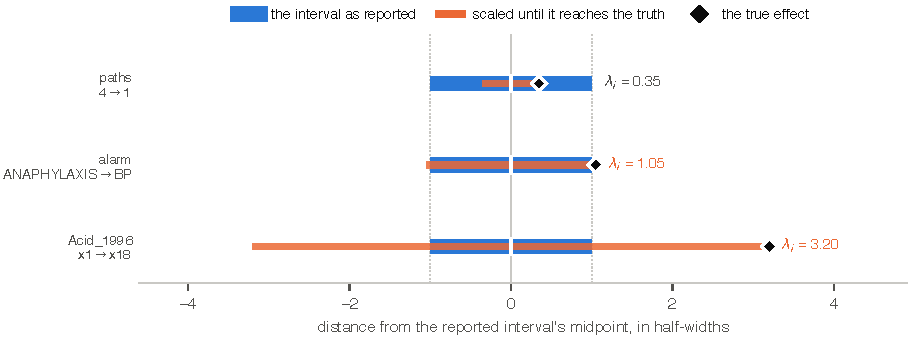
\includegraphics[width=\textwidth]{figs/f1_lambda.pdf}
\caption{Three real problems from the one-wrong-claim condition, at $n = 1000$, drawn on a common
scale where the reported interval always runs from $-1$ to $+1$. The factor $\lambda_i$ is what the
interval would have to be multiplied by, about its own midpoint, to reach the true effect.}
\end{figure}

\subsection{Step 2. One factor for the whole cell}

Now do that for every problem in the cell and every random draw. A cell of Panel B at one wrong
claim holds 359 problems and twenty draws each, so 7{,}180 of these numbers.

Sort them and take the 95th percentile. Call it $\lambda^{*}$. By construction, multiplying every
interval in the cell by $\lambda^{*}$ makes 95\,\% of them contain the truth. That is the single
factor that buys honest coverage for this procedure on this population.

\begin{figure}[h]
\centering
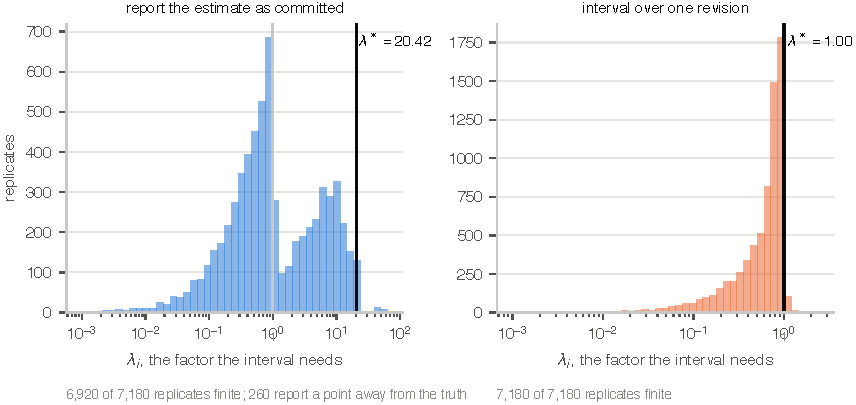
\includegraphics[width=\textwidth]{figs/f2_calibration.pdf}
\caption{The distribution of $\lambda_i$ over all 7{,}180 replicates of the one-wrong-claim cell,
for two procedures. Reporting the estimate as committed is bimodal: one group of problems is
roughly right, and a second group sits an order of magnitude away, which is what one false claim
does. Its 95th percentile is 20.4. The interval over one revision needs no stretching at all, so
its factor is 1.00.}
\end{figure}

The shape on the left is the finding behind the whole column. Committing to the analyst's graph does
not produce intervals that are a bit too narrow. It produces two populations: problems where the
false claim did not matter, and problems where the reported effect is simply somewhere else.

\subsection{Step 3. From the factor to a width, and then to a ratio}

Multiply each interval by $\lambda^{*}$ and average the resulting widths. That is the calibrated
width, in effect units. Then divide by the calibrated width of the procedure that discards the
knowledge entirely. The result is the number printed in the cell.

\begin{quoting}
At one wrong claim, $n = 1000$, semi-synthetic panel:

\smallskip
\begin{tabular}{@{}lrrr@{}}
\toprule
procedure & $\lambda^{*}$ & mean half-width & calibrated width \\
\midrule
report the estimate as committed & 20.416 & 0.3855 & 15.7397 \\
interval over one revision & 1.000 & 1.3064 & 2.6129 \\
discard the knowledge, whole class & 1.000 & 1.5361 & 3.0721 \\
\bottomrule
\end{tabular}

\smallskip
$15.7397 / 3.0721 = 5.123$. \qquad $2.6129 / 3.0721 = 0.851$.
\end{quoting}

Those are the two numbers in the middle column of the table. So the row that reports the estimate as
committed is a narrow interval, mean half-width 0.39 against 1.54 for the whole class, and it is the
most expensive of the three once you require it to be right.

\begin{figure}[h]
\centering
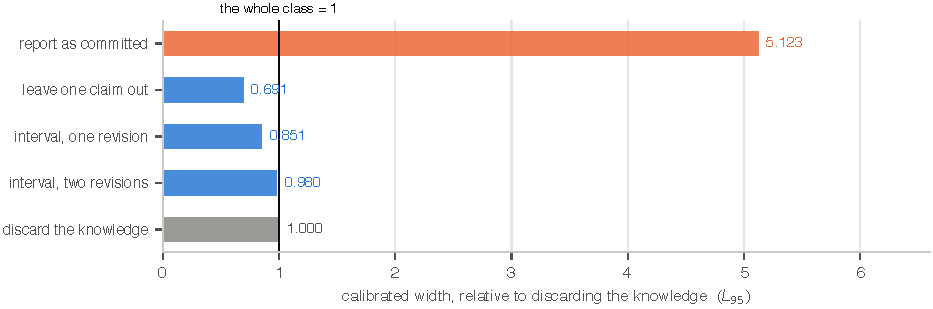
\includegraphics[width=\textwidth]{figs/f3_ratio.pdf}
\caption{The middle column of Panel B, as calibrated widths relative to discarding the knowledge.
Anything to the right of the line costs more than using no background knowledge at all.}
\end{figure}

\subsection{Why a number can exceed one, and what that means}

A procedure earns a number above one when its interval is narrow and centred in the wrong place.
Stretching happens about the interval's own midpoint, so a displaced midpoint has to be compensated
on both sides. Committing to a graph built on a false claim puts the midpoint at the effect that
graph implies, which is a different quantity from the one being estimated.

\begin{figure}[h]
\centering
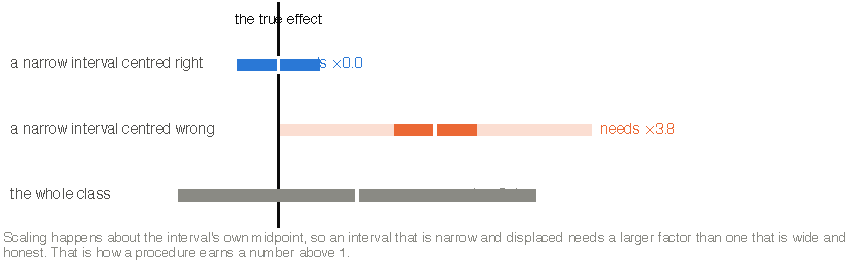
\includegraphics[width=\textwidth]{figs/f5_why_above_one.pdf}
\caption{Three intervals and the factor each needs. A narrow interval centred on the truth is cheap.
A narrow interval centred away from it is the most expensive object in the table. Schematic.}
\end{figure}

A value above one is therefore a strong statement, and it is the statement the table is making about
current practice: at one wrong claim, an analyst who reports the estimate their graph produced is
worse off than an analyst who never elicited any knowledge, by a factor of five.

\subsection{Reading the whole panel}

\begin{figure}[h]
\centering
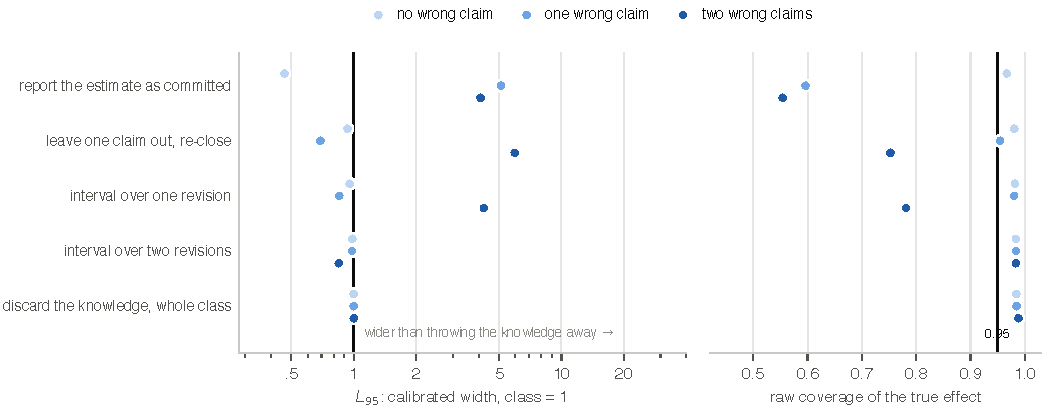
\includegraphics[width=\textwidth]{figs/f4_panelB.pdf}
\caption{Panel B as a chart. Left: the calibrated width of each procedure, with the whole class at
one. Right: the raw coverage each procedure achieved before any calibration. Semi-synthetic
parameters on published structures, $n = 1000$; 391, 359 and 131 problems over 23, 23 and 9
networks.}
\end{figure}

Five things are worth saying out loud from that picture.

The first column is a defeat and it has to be. When nothing is wrong, the committed report needs
0.464 and the interval over one revision needs 0.957, so the insurance costs about twice the width
when the knowledge is correct. A table in which the proposed method wins every column is a design
error, and a reviewer reads it as one.

One wrong claim is bought back cheaply. The committed report drops to 0.597 coverage, and the
interval over one revision covers 0.980 while needing 0.851 of the class width. It is also 15\,\% narrower than the procedure that uses no knowledge at all, which is the
reason the knowledge was worth eliciting in the first place.

Two wrong claims need two retractions. The interval over one revision fails at two wrong claims
(coverage 0.781, and a calibrated width of 4.234 that is worse than the class), and the interval
over two pays. The depth of the budget has to match the number of errors; there is no budget that is
free.

Retracting one claim far from the query is not the bargain it looks like. That row is the matched
negative control, and it costs more than doing nothing while buying four points of coverage. On the
semi-synthetic panel it is not inert, because a far retraction still propagates into the component
through the orientation rules. That prediction was recorded as partial rather than supported.

The free screen and the interval agree at this depth. The leave-one-out screen needs 0.691 at one
wrong claim against the interval's 0.851, and fails at two wrong claims exactly where the interval
over one revision fails. That is the tie the paper states as a property rather than hiding.

\subsection{Two cautions about the panel as printed}

\textbf{The three columns are three populations.} A problem enters the one-wrong-claim column only
if it has at least one local claim to falsify, and the two-wrong-claim column only if it has two and
they can be reversed consistently. That is why the counts fall from 391 to 359 to 131 and the
network count from 23 to 9. The populations are nested, and the counts are printed under the panel
for that reason. Comparing down a column is exact; comparing across a row is comparing three
different problem sets.

\textbf{The numbers depend on the sample size, and the table shows only one.} At $n = 20\,000$ the
committed report's number rises from 5.123 to 14.368, because more data makes a wrongly centred
interval narrower without moving it. The relative price of the interval improves from 0.851 to
0.758. The direction is the same and the magnitudes are not, so the sample size belongs in the
caption of any quotation.

\subsection{The definitions behind the row names}

\begin{center}\small
\begin{tabular}{@{}p{4.3cm}p{11.7cm}@{}}
\toprule
row & what the procedure does \\
\midrule
report the estimate as committed & Take the analyst's graph, read off the adjustment set the
generalised criterion gives, fit, report the ordinary 95\,\% interval. Where the graph commits to no
set, report the band over its own possible parent sets, which is the budget-zero interval. This is
the documented practice, and it is the default the table is arguing against \\
\addlinespace
leave one claim out, re-close, widen if it changes & For each claim in turn, drop it, close the graph
again under the orientation rules, recompute the committed set. If any of them changes the answer,
report the interval over one revision; otherwise report the committed estimate \\
\addlinespace
interval over one revision & The union of the estimates over every knowledge state within one
elementary revision of the analyst's claims, taken as an interval \\
\addlinespace
interval over two revisions & The same over two revisions \\
\addlinespace
discard the knowledge, whole class & The interval over every adjustment set the equivalence class
admits, using no background knowledge. It is the denominator of every cell, so it is 1.000 by
construction, and its raw coverage is printed to show that it is honest rather than merely wide \\
\bottomrule
\end{tabular}
\end{center}

Every row uses the same estimator and the same data. What differs between rows is only how many
revisions of the asserted knowledge the reported interval is willing to tolerate.

\clearpage
\section{T3 in full: all twenty-six rows}

This is the whole table, generated from the stored results rather than transcribed. The knowledge
condition is the recovering set, the estimates are at $n = 20\,000$ with the first seed, and the
population interval behind each band is in the source file. Three declared queries are excluded and
they are listed under the table with the reason.

\begin{landscape}
\begin{table}[p]
\centering
\footnotesize
\setlength{\tabcolsep}{3pt}
\caption*{\textbf{T3.} Sensitivity reports on twenty-six named analyses. $|K|$ is the number of claims the analyst asserts, with the number inside the treatment's own component in parentheses. The two interval columns are the union of the estimate over every knowledge state within one and two elementary revisions of those claims. $r_0$ is the null radius, the number of revisions after which the interval contains zero, from the population, from the band at the first seed, and as the range over twenty seeds. $r_{\mathrm{val}}$ is the breakdown radius, the number of revisions after which the committed adjustment set stops being valid. The last column names the claims whose retraction first opens the interval to zero, in the source's own variable names. Knowledge: the recovering set; estimates at $n = 20\,000$, first seed.}
\begin{tabular}{@{}llccl cc l c l@{}}
\toprule
network & query & $|K|$ & true & estimate [95\,\%] & one revision & two revisions
 & $r_0$ pop / seed / range & $r_{\mathrm{val}}$ & first breaking claims \\
\midrule
\multicolumn{10}{@{}l}{\itshape Published analyses: the treatment and the outcome are the ones the source paper declares.}\\[1pt]
Acid\_1996 & x3 $\to$ x15 & 1 (0) & $-2.169$ & $-2.176$ [$-2.203$, $-2.149$] & [$-2.226$, $-2.147$] & [$-2.226$, $-2.147$] & never / $>$3 / $>$3 & never & -- \\
Didelez\_2010 & HRT $\to$ TCI & 1 (0) & $-0.586$ & $-0.586$ [$-0.599$, $-0.572$] & [$-0.604$, $-0.568$] & [$-0.604$, $-0.568$] & never / $>$3 / $>$3 & never & -- \\
Kampen\_2014 & SUS $\to$ EGC & 3 (0) & $-0.643$ & $-0.647$ [$-0.663$, $-0.630$] & [$-0.663$, $-0.630$] & [$-0.663$, $-0.630$] & never / $>$3 / $>$3 & never & -- \\
Polzer\_2012 & ToothLoss $\to$ Mortality & 5 (0) & $\phantom{-}1.193$ & $\phantom{-}1.190$ [$\phantom{-}1.183$, $\phantom{-}1.197$] & [$\phantom{-}1.128$, $\phantom{-}1.208$] & [$\phantom{-}1.128$, $\phantom{-}1.208$] & never / $>$3 / $>$3 & $>$3 & -- \\
Sebastiani\_2005 & EDN1.3 $\to$ EDNI1.7 & 7 (0) & $-1.212$ & $-1.209$ [$-1.219$, $-1.199$] & [$-1.234$, $-1.179$] & [$-1.234$, $-1.179$] & never / $>$3 / $>$3 & $>$3 & -- \\
Shrier\_2008 & WarmUpExercises $\to$ Injury & 2 (0) & $-1.351$ & $-1.348$ [$-1.358$, $-1.339$] & [$-1.431$, $-1.228$] & [$-1.431$, $-1.228$] & never / $>$3 / $>$3 & never & -- \\
Thoemmes\_2013 & x $\to$ y & 1 (1) & $-0.923$ & $-0.913$ [$-0.928$, $-0.898$] & [$-1.002$, $-0.871$] & [$-1.002$, $-0.871$] & never / $>$3 / $>$3 & never & -- \\
mediator & X $\to$ Y & 3 (3) & $-2.603$ & $-2.600$ [$-2.623$, $-2.576$] & [$-2.623$, $-1.109$] & [$-2.623$, $\phantom{-}0.000$] & 2 / 2 / 2 & 1 & Z$\to$I \,/\, Z$\to$X \\
paths & E $\to$ D & 1 (0) & $\phantom{-}1.194$ & $\phantom{-}1.193$ [$\phantom{-}1.188$, $\phantom{-}1.197$] & [$\phantom{-}1.169$, $\phantom{-}1.216$] & [$\phantom{-}1.169$, $\phantom{-}1.216$] & never / $>$3 / $>$3 & never & -- \\
\addlinespace
\multicolumn{10}{@{}l}{\itshape Networks with coefficients fitted to real data: the frame rows whose analyst graph commits to a set.}\\[1pt]
ecoli70 & asnA $\to$ aceB & 10 (1) & $\phantom{-}0.547$ & $\phantom{-}0.542$ [$\phantom{-}0.511$, $\phantom{-}0.572$] & [$-0.011$, $\phantom{-}0.572$] & [$-0.011$, $\phantom{-}0.572$] & 1 / 1 / 1..$>$3 & 1 & asnA$\to$icdA \\
ecoli70 & b1191 $\to$ yfaD & 10 (1) & $-0.098$ & $-0.097$ [$-0.105$, $-0.089$] & [$-0.114$, $\phantom{-}0.029$] & [$-0.114$, $\phantom{-}0.029$] & 1 / 1 / 1 & 1 & b1191$\to$fixC \\
ecoli70 & cspG $\to$ hupB & 10 (7) & $\phantom{-}0.257$ & $\phantom{-}0.265$ [$\phantom{-}0.246$, $\phantom{-}0.283$] & [$\phantom{-}0.003$, $\phantom{-}0.308$] & [$\phantom{-}0.003$, $\phantom{-}0.308$] & 1 / $>$3 / 1..$>$3 & 1 & -- \\
ecoli70 & pspB $\to$ nmpC & 10 (7) & $-0.108$ & $-0.100$ [$-0.118$, $-0.082$] & [$-0.531$, $\phantom{-}0.026$] & [$-0.531$, $\phantom{-}0.026$] & 1 / 1 / 1..3 & 1 & pspB$\to$pspA \\
ecoli70 & eutG $\to$ lacY & 10 (1) & $\phantom{-}0.309$ & $\phantom{-}0.309$ [$\phantom{-}0.279$, $\phantom{-}0.338$] & [$\phantom{-}0.277$, $\phantom{-}0.377$] & [$\phantom{-}0.277$, $\phantom{-}0.377$] & never / $>$3 / $>$3 & 1 & -- \\
arth150 & 100 $\to$ 245 & 29 (3) & $\phantom{-}1.535$ & $\phantom{-}1.534$ [$\phantom{-}1.527$, $\phantom{-}1.542$] & [$\phantom{-}0.000$, $\phantom{-}1.545$] & [$\phantom{-}0.000$, $\phantom{-}1.545$] & 1 / 1 / 1 & 1 & 100$\to$245 \\
arth150 & 81 $\to$ 464 & 29 (10) & $\phantom{-}0.256$ & $\phantom{-}0.184$ [$\phantom{-}0.118$, $\phantom{-}0.250$] & [$\phantom{-}0.097$, $\phantom{-}0.265$] & [$\phantom{-}0.097$, $\phantom{-}0.265$] & $>$3 / $>$3 / $>$3 & $\geq$2 & -- \\
magic-niab & G1853 $\to$ G43 & 8 (1) & $-0.039$ & $-0.028$ [$-0.038$, $-0.017$] & [$-0.038$, $\phantom{-}0.020$] & [$-0.038$, $\phantom{-}0.020$] & 1 / 1 / 1..$>$3 & 1 & G1853$\to$G311 \\
magic-niab & G311 $\to$ G43 & 8 (1) & $-0.255$ & $-0.251$ [$-0.259$, $-0.244$] & [$-0.260$, $\phantom{-}0.000$] & [$-0.260$, $\phantom{-}0.000$] & 1 / 1 / 1 & 1 & G1853$\to$G311 \\
magic-niab & G418 $\to$ FUS & 8 (2) & $\phantom{-}0.003$ & $-0.003$ [$-0.015$, $\phantom{-}0.010$] & [$-0.022$, $\phantom{-}0.011$] & [$-0.022$, $\phantom{-}0.011$] & 1 / 0 / 0..1 & 1 & -- \\
magic-niab & G1217 $\to$ FT & 8 (1) & $\phantom{-}0.068$ & $\phantom{-}0.015$ [$-0.029$, $\phantom{-}0.060$] & [$-0.031$, $\phantom{-}0.131$] & [$-0.031$, $\phantom{-}0.131$] & never / 0 / 0..$>$3 & 1 & -- \\
magic-niab & G1217 $\to$ YLD & 8 (1) & $\phantom{-}0.009$ & $\phantom{-}0.011$ [$\phantom{-}0.003$, $\phantom{-}0.018$] & [$\phantom{-}0.004$, $\phantom{-}0.021$] & [$\phantom{-}0.004$, $\phantom{-}0.021$] & never / $>$3 / 0..$>$3 & 1 & -- \\
magic-irri & G1378 $\to$ SUB & 10 (1) & $-0.035$ & $-0.031$ [$-0.044$, $-0.017$] & [$-0.048$, $\phantom{-}0.021$] & [$-0.048$, $\phantom{-}0.021$] & 1 / 1 / 1 & 1 & G1378$\to$G1311 \\
magic-irri & G3212 $\to$ FT & 10 (2) & $\phantom{-}0.004$ & $-0.025$ [$-0.070$, $\phantom{-}0.020$] & [$-0.143$, $\phantom{-}0.008$] & [$-0.143$, $\phantom{-}0.008$] & 1 / 0 / 0..1 & 1 & -- \\
magic-irri & G3925 $\to$ GTEMP & 10 (1) & $\phantom{-}0.000$ & $\phantom{-}0.001$ [$-0.034$, $\phantom{-}0.036$] & [$-0.131$, $\phantom{-}0.038$] & [$-0.131$, $\phantom{-}0.038$] & 1 / 0 / 0 & 1 & -- \\
magic-irri & G4145 $\to$ G3222 & 10 (2) & $-0.020$ & $-0.015$ [$-0.025$, $-0.004$] & [$-0.026$, $\phantom{-}0.026$] & [$-0.026$, $\phantom{-}0.026$] & 1 / 0 / 0..1 & 1 & -- \\
magic-irri & G4156 $\to$ CHALK & 10 (2) & $\phantom{-}0.404$ & $\phantom{-}0.501$ [$\phantom{-}0.361$, $\phantom{-}0.641$] & [$-0.154$, $\phantom{-}0.664$] & [$-0.154$, $\phantom{-}0.664$] & 1 / 1 / 1..$>$3 & 1 & G4156$\to$G4145 \\
\bottomrule
\end{tabular}
\end{table}
\end{landscape}


\noindent Excluded, with the reason: M-bias, E on D, because the published diagram is not a
directed acyclic graph; Schipf 2010, TT on T2DM, because the outcome is not a possible descendant of
the treatment, so there is no effect to report; confounding, E on D, because the treatment has no
undirected edge, so no claim of the analyst's bears on it.

\subsection{What the table says once you have read it twice}

The published analyses are robust and the sampled ones are not. Of the nine declared queries that
can be certified, eight are unbroken by any retraction down to depth three: their interval is a
point, their radius is never reached, and no claim the analyst made is load-bearing. The one
exception is mediator, a four-node textbook diagram. Below the rule, on the four networks with
fitted coefficients, sixteen of seventeen informative queries break at the first retraction.

The reason is mechanical and it belongs in the paper. A query enters the sampled frame only if some
retraction changes the validity of the committed set, so a query that no retraction can touch is
rejected before it is measured. The population the method is evaluated on is therefore close to the
complement of the queries these source papers exist to answer, which is an applicability statement
rather than a result.

The radius is almost always one. Across the whole table $r_{\mathrm{val}}$ takes the value one on
every informative row except mediator. In practice the quantity is a pointer to a single claim
rather than a graded scale.

The null radius and the breakdown radius are different numbers and they disagree. On mediator the
set stops being valid after one revision while the interval only reaches zero after two. On several
fitted rows the null radius read from the band at a single seed is zero, meaning the reported
interval already contained zero before any retraction: at that sample size there was no conclusion
to break. The range column exists because that reading moves with the seed, so any sentence about
the null radius has to carry which of the three readings it uses.

One retraction is not a small perturbation. On sixteen of the seventeen informative rows the
interval after retracting one claim is the whole class interval, to four decimals. All the
identifying power the knowledge supplies sits in a single claim, and withdrawing it returns the
analyst to where they would have been with no background knowledge at all. That fact is what the
figure in the next section is built around.

\clearpage
\section{The figure for T3}

\subsection{The constraint nobody wrote down}

The obvious figure for a sensitivity analysis is a curve: the conclusion on one axis, the amount of
assumed knowledge withdrawn on the other, and a smooth frontier where the conclusion gives out. That
is the shape Rosenbaum's plots have, and it is the shape the paper's own figure rule went looking
for: a row whose interval stays flat for a while and then breaks.

That rule returned nothing. No query under the recovering set or under truthful knowledge has both
radii in the middle of the range on a network with real coefficients, and the rows that do have them
widen by a factor of twenty-seven to thirty-four before they break, so the plateau never happens.

The reason is in the data and it is the most important design fact here. The curve is not smooth.
It is a single step.

\begin{figure}[h]
\centering
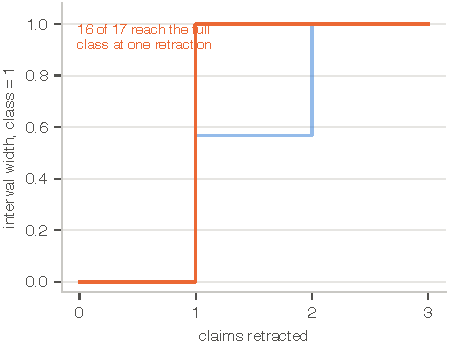
\includegraphics[width=.48\textwidth]{figs/f7_T3_steps.pdf}
\caption{Interval width against the number of claims retracted, one line per analysis, each
normalised to the width of the interval that uses no knowledge. Sixteen of the seventeen informative
analyses go from a point to the full class in one step. The exception is the textbook mediator,
which takes two.}
\end{figure}

Any figure that draws a frontier on this data is drawing something that is not there. The honest
encodings are the ones that treat the budget as what it is, a small integer, and put their effort
into showing what the step costs rather than pretending it is gradual.

\subsection{Five candidates}

\subsubsection*{F-A. The one-claim cliff}

Every analysis on one axis, each normalised so that the effect the analyst reported sits at one and
the null sits at zero. Three marks per row: the reported estimate, the interval after retracting one
claim, and the interval with no knowledge at all. The claim that does it is named in its own column.

\begin{figure}[h]
\centering
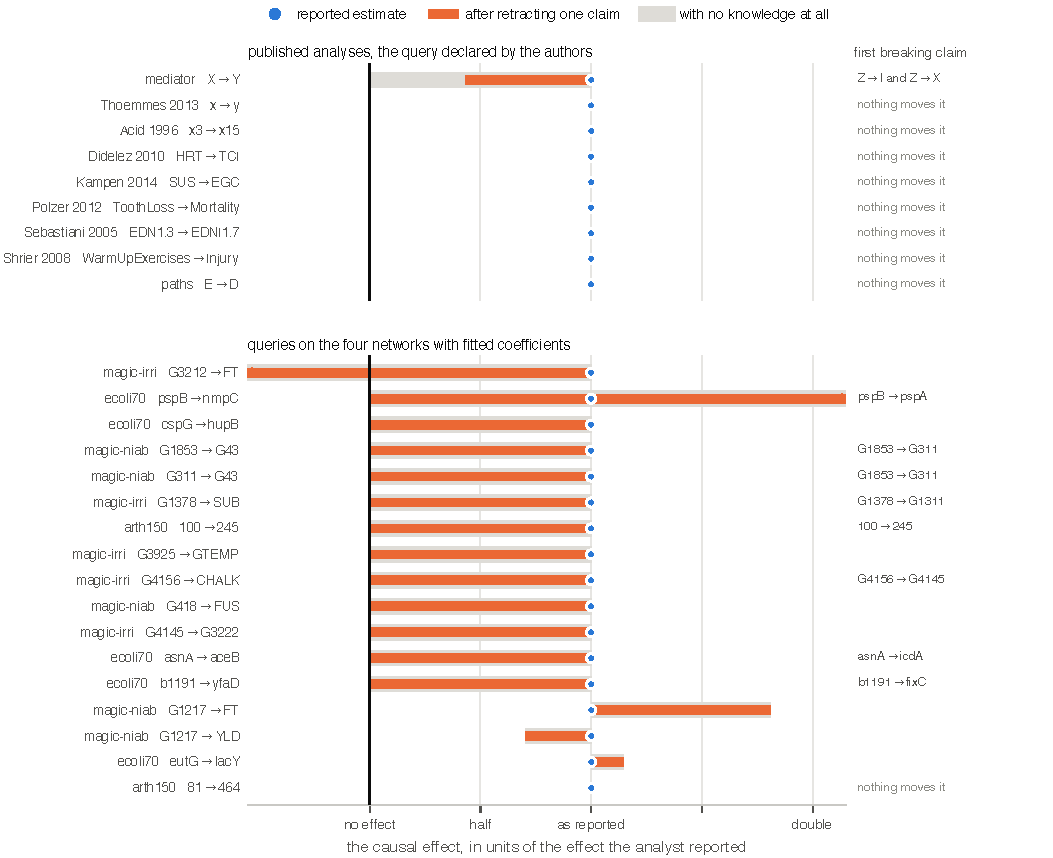
\includegraphics[width=\textwidth]{figs/f6_T3_dumbbell.pdf}
\caption{F-A, drawn from the twenty-six rows of T3. Normalising by the reported effect puts every
analysis on one scale and makes the pattern arithmetic rather than rhetorical: below the rule, one
retraction opens the interval from a point at the reported effect to everything between that and
zero. Where only the orange bar is visible, the grey one is underneath it, which is the finding.}
\end{figure}

What it shows: the reported effect and no effect become indistinguishable after one revision, on
every query drawn from the sampled frame, and on none of the queries the source papers declared.
Both halves are load-bearing and they sit in one picture.

What it costs: it needs a normalisation, and a reader has to accept that dividing by the reported
effect is fair. Two rows run off the axis and carry an arrow.

\subsubsection*{F-B. The step law}

The figure above, in the section on the constraint. Width against budget, one line per analysis.

What it shows: that the quantity is a step and not a frontier, which is the honest correction to
what a reader expects.

What it costs: sixteen of the lines are the same line. It is one fact, and a sentence carries it as
well as a panel does.

\subsubsection*{F-C. The state strip}

One row per analysis, one cell per budget, coloured by whether the interval at that budget still
determines the sign of the effect. No normalisation and no continuous axis, so nothing is implied
about magnitude.

\begin{figure}[h]
\centering
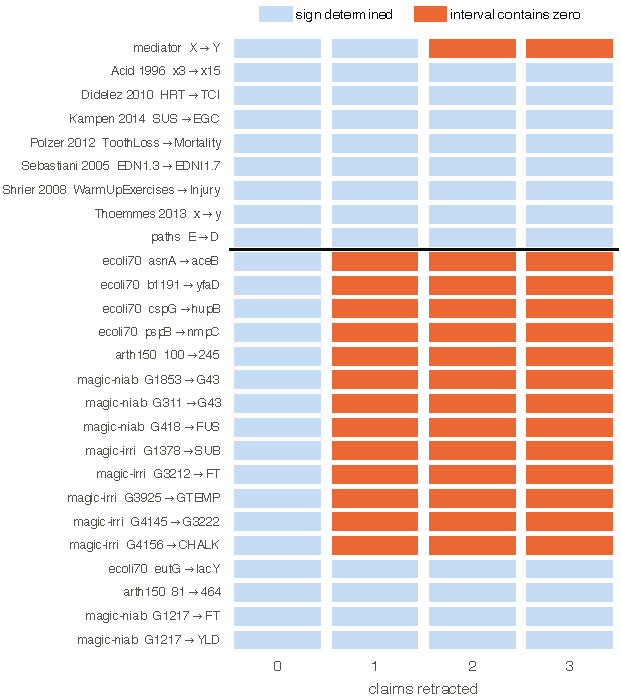
\includegraphics[width=.42\textwidth]{figs/f8_T3_strip.pdf}
\caption{F-C. The state of each conclusion at each budget, read from the stored null radius rather
than recomputed. Above the rule, the analyses whose queries the source papers declared.}
\end{figure}

What it shows: the discreteness, honestly, and the contrast between the declared queries and the
sampled ones at a glance.

What it costs: it drops the magnitude entirely. A reader learns that the conclusion goes and not
that it goes all the way to zero, which is the part that should alarm them.

\subsubsection*{F-D. The paradigm card}

One analysis, three lanes: what the analyst reports, what they would report having withdrawn one
named claim, and what they would report having asserted nothing.

\begin{figure}[h]
\centering
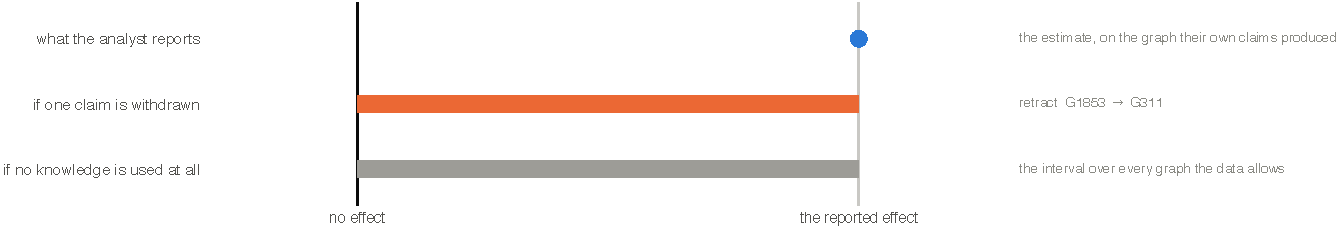
\includegraphics[width=\textwidth]{figs/f9_T3_card.pdf}
\caption{F-D. A single query on a network with fitted coefficients. The second lane and the third
are the same interval, which is what it means for the conclusion to rest on one claim.}
\end{figure}

What it shows: the object, the quantity and the sentence a practitioner would say, in one picture
that needs no axis labels to be understood.

What it costs: it is one row of a twenty-six-row table, so on its own it is an illustration. A
reviewer asks immediately whether it was chosen.

\subsubsection*{F-E. The cliff with its population}

F-A, with the distribution of the radius over every query in the corpus beside it, so that the named
analyses can be located in the population they were drawn from.

\begin{figure}[h]
\centering
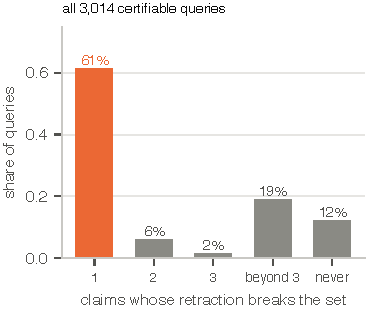
\includegraphics[width=.40\textwidth]{figs/f10_T3_population.pdf}
\caption{The right-hand panel of F-E: the breakdown radius over all 3{,}014 certifiable queries,
eleven knowledge conditions, 27 networks. The last two bars are queries whose set survives every
retraction the search reached, and queries no retraction can break at all. On 61\,\% of them the
committed set rests on a single claim.}
\end{figure}

What it shows: where the twenty-six named analyses sit in the population they were drawn from. They
are a selection, and the next section measures which of their columns that selection moved and which
it left alone.

What it costs: two populations in one float, which has to be said in the caption and read carefully.

\subsection{The recommendation}

\begin{verdict}
\textbf{Draw F-A, and put the population panel of F-E beside it.} Use F-D as the page-one teaser,
with a different query from the one F-A leads with, so the two do not restate each other. Keep F-B
as a sentence in the results and F-C in the appendix.
\end{verdict}

The argument for F-A over the others is that it is the only candidate that carries all three things
a reader needs at once. It shows the quantity, because the bar is the interval at one retraction.
It shows the consequence in the units the analyst reports in, because the axis is their own effect.
And it shows the comparison, because the grey bar behind is what they would have had with no
knowledge at all, and on sixteen rows of seventeen it is hidden underneath the orange one.

That last point is worth stating as the caption's one sentence, because it is the finding that the
table makes and the curve figure cannot: \emph{on these analyses, retracting a single claim returns
the analyst to the interval they would have had if they had asserted nothing}.

\subsection{Can this be the paper's main contribution}

It can be the main \emph{figure}. Two cautions before it becomes the main \emph{claim}.

The first is selection, and the next section measures it. The rows in the lower panel were chosen by
a rule that puts queries with a finite null radius first, so the null radius column of T3 is not
representative: 76\,\% of the printed rows against 43\,\% of the eligible ones. The width claim the
figure is built on is untouched by that rule, holding on 26 of 26 eligible queries and on 211 of 226
across the corpus. So the figure is safe and the caption must still say how the rows were drawn.

The second is that the figure is read as showing the null radius while the paper's headline quantity
is the breakdown radius. They coincide on most of these rows and they are different objects, and the one
analysis where they differ is the textbook one. A figure built on the interval reaching zero is
making a claim about conclusions; a figure built on the set ceasing to be valid is making a claim
about validity. Choose which, and say so in the axis label rather than in the text.

With both of those handled, the figure carries the paper. A reviewer who has read only the abstract
can look at it and see what the method measures, what it costs, and why the answer is uncomfortable.

\clearpage
\section{Why twenty-six rows, and what the other networks say}

T3 is not the corpus. It is a selection from it, made by two rules, and only one of them is
defensible. This section prints the funnel, names both rules, and measures what the selection did
to the numbers the table reports.

\subsection{The funnel, under the recovering set}

\begin{center}\small
\begin{tabular}{@{}rp{11.9cm}@{}}
\toprule
& stage \\
\midrule
39 & networks parsed from the corpus \\
33 & have a frame, meaning at least one treatment beside an undirected edge with the outcome a
possible descendant \\
27 & are swept. The six that are not exceed 500 nodes, or all their chain components exceed the
questionnaire cap \\
80{,}132 & candidate treatment--outcome pairs, built from observables alone \\
648 & pairs sampled into the frame, capped at twenty per network \\
537 & rows under the recovering set: 528 sampled plus 9 the source papers declare. All are
certifiable \\
234 & of those say the outcome cannot descend from the treatment on the analyst's own graph, so
the effect is zero and there is no adjustment set to report on \\
\textbf{303} & \textbf{commit to an adjustment set. This is the population a sensitivity report
could be written for: 9 declared and 294 sampled, over 27 networks} \\
\midrule
26 & are printed in T3 \\
\bottomrule
\end{tabular}
\end{center}

So the table shows 9 of the 9 declared queries and 17 of the 294 sampled ones, which is 5.8\,\% of
the eligible population. The 277 that are missing are missing for two different reasons.

\subsection{Rule one: only four networks have real coefficients}

Of the 27 swept networks, four carry coefficients fitted to real data: \texttt{ecoli70},
\texttt{arth150}, \texttt{magic-niab} and \texttt{magic-irri}. The other 23 carry structure from a
published source and parameters we drew ourselves, uniform in a fixed range with unit noise.

A sensitivity report on a named analysis prints an effect size and an interval. On a
semi-synthetic network those numbers are ours, not the field's, so the row would read as a report
on a real analysis while carrying an invented effect. That is why the other 23 networks contribute
257 eligible rows and none of them appear.

This rule is defensible and it should be printed in the caption, which it currently is not. Those
23 networks are not absent from the paper: they are the population behind the price table, the
certificate ladder and the funnel, where only the structure matters and the parameters are a
nuisance. They are absent from this one table, because this one table is about named effects.

\subsection{Rule two: the first five per network, and it is not defensible as written}

On the four remaining networks, 37 queries commit to a set and are therefore eligible. The table
takes five per network, which is 17 of 37, because \texttt{arth150} only has two.

The 20 that were dropped are 9 on \texttt{magic-niab}, 8 on \texttt{magic-irri} and 3 on
\texttt{ecoli70}. The cap is arbitrary and a reviewer will say so, but the cap is not the problem.
The ordering is.

\begin{verdict}
The eligible queries are sorted so that those with a finite null radius come first, and then the
first five are taken. A finite null radius means the interval reaches zero within the search depth,
which is the outcome the table exists to illustrate.

The effect is measurable. Across the 37 eligible queries, 16 have a finite null radius, which is
43\,\%. Among the 17 the table prints, 13 do, which is 76\,\%. Among the 20 it drops, 3 do, which
is 15\,\%.
\end{verdict}

So the null-radius column of T3 is not representative of the population it is drawn from, and the
fix is one line: sort by frame index alone, or print all 37. Either is honest and the second is
better, because the inclusion rule then has nothing in it that a reader has to trust.

\subsection{What the selection did not do}

The claim the figure of the previous section is built on survives the audit, and it survives it
comfortably.

\begin{center}\small
\begin{tabular}{@{}lccc@{}}
\toprule
population & queries & informative & of those, one retraction reaches the whole class \\
\midrule
printed in T3 & 17 & 16 & 16 of 16 \\
dropped by the cap & 20 & 10 & 10 of 10 \\
the full eligible pool & 37 & 26 & 26 of 26 \\
every committed row, 27 networks & 294 & 226 & 211 of 226 \\
\bottomrule
\end{tabular}
\end{center}

On every query the table could have shown, and on 93\,\% of every query in the corpus, retracting a
single claim returns the interval to the one the analyst would have had with no background knowledge
at all. The cap did not manufacture that pattern; it is the pattern of the corpus.

\begin{figure}[p]
\centering
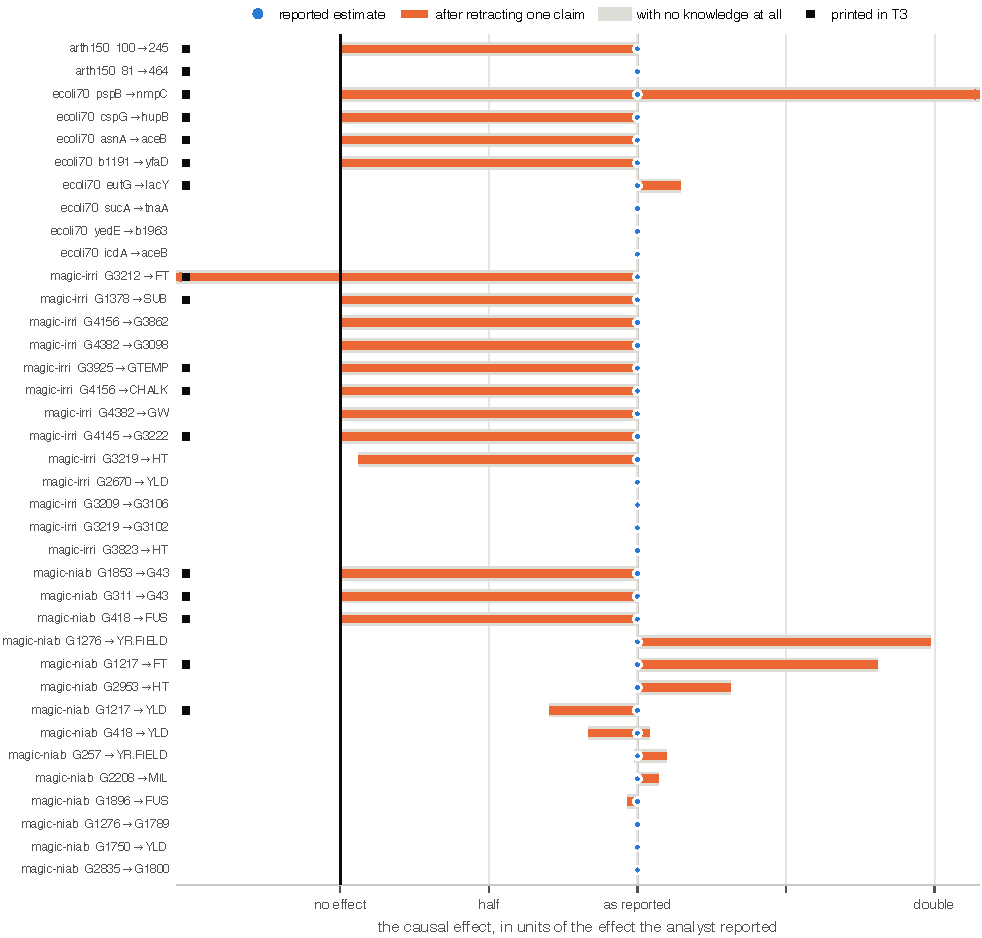
\includegraphics[width=\textwidth]{figs/f11_pool_dumbbell.pdf}
\caption{The recommended figure drawn on all 37 eligible queries rather than the seventeen T3
prints, with the printed ones marked. Eleven rows carry no bar at all: on those the class already
pins the effect and no retraction moves it, which is the honest counterweight and is invisible in
the table as printed.}
\end{figure}

\subsection{What to change}

Three things, and none of them is expensive.

Print the inclusion rule in T3's caption, naming both the real-coefficient restriction and the cap,
and give the count of eligible queries beside the count shown. Instance selection is this form's
whole attack surface and the only defence is stating the rule.

Remove the finite-null-radius term from the sort. The cap can stay at five per network if space
demands it, but taking the first five in frame order costs nothing and removes the bias from the
null-radius column.

Draw the figure on the 37, not the 17. It is the same picture, it is one page, it needs no
inclusion rule at all beyond the real-coefficient restriction, and it contains the eleven rows where
nothing moves, which the table currently hides.

\clearpage
\section{Why one revision and two revisions print the same interval}

On 25 of the 26 rows the two interval columns are identical, in the printed band and in the
population. The only row where they differ is \texttt{mediator}. The reason is structural, and it is the same
fact the figure is built on seen from another angle.

The interval over $r$ revisions is a union over knowledge states, so it grows with $r$ and it is
bounded above by the interval over the whole equivalence class. The class interval is a ceiling that
no amount of retracting can pass, because retracting all of the knowledge is exactly what the class
already assumes. So the two columns can only differ on a row where the first revision has not yet
reached that ceiling.

\begin{center}\small
\begin{tabular}{@{}rp{12.6cm}@{}}
\toprule
rows & what the second revision adds, and why \\
\midrule
9 & The class interval is a point. The effect is identified by the data alone, no asserted claim
bears on it, and every budget returns the same sampling interval. Seven of these are declared
queries whose claims all sit outside the treatment's component \\
\addlinespace
16 & The first revision already returns the whole class, to four decimals. The ceiling is reached at
$r = 1$, so $r = 2$ has nothing left to add \\
\addlinespace
1 & mediator. The first revision covers 57\,\% of the class and the second saturates it.
This is the only row in the table where the second column carries information \\
\bottomrule
\end{tabular}
\end{center}

The mechanism behind the sixteen is the breakdown radius itself. The extreme of the class is
attained by some knowledge state, and reaching it requires retracting the smallest set of claims
that reaches it. That set is a single claim on 141 of the 157 queries with an exact certificate, and
on every one of those the union at $r = 1$ already contains the extreme. A second retraction can
only add states that were already inside.

\subsection{The same count on all 303 rows}

The exhaustive table lets the question be asked of the whole population rather than of the
twenty-six.

\begin{center}\small
\begin{tabular}{@{}rp{12.6cm}@{}}
\toprule
rows & of the 303 queries that commit to an adjustment set \\
\midrule
281 & print the same interval at one and at two revisions, in the band and in the population,
which is 92.7\,\% \\
76 & have a class interval that is a point: no asserted claim bears on the query at any budget \\
205 & reach the whole class at the first revision \\
22 & have a first revision strictly inside the class, and on 20 of those the second revision
widens the interval \\
\bottomrule
\end{tabular}
\end{center}

So the second column carries information on 20 queries in 303. Where those 20 sit is the part worth
noticing: they are on insurance, Polzer 2012, Kampen 2014, sachs, Schipf 2010 and mediator. Every
one of those networks except mediator is excluded from the printed T3 by the real-coefficient rule.
The column looks empty in T3 because T3 drops the networks on which it is full.

\begin{verdict}
\textbf{What to do with the column.} Replace \emph{two revisions} with \emph{no knowledge at all},
the class interval. On the sixteen saturated rows the reader then sees two identical intervals side
by side, and that identity is the finding rather than a redundancy. On mediator they differ,
and the difference is legible for the first time. The exhaustive table below prints all three
columns so the substitution can be checked.
\end{verdict}

\clearpage
\section{The exhaustive table}

Both selection rules removed. Every query under the recovering set whose analyst graph commits to an
adjustment set: 303 rows over all 27 swept networks, with the four fitted-coefficient networks and
the 23 semi-synthetic ones in separate blocks and a provenance column, so the rule that was dropped
is visible rather than applied. A bullet marks the 26 rows the printed T3 selects.

Every cell that the printed T3 also shows was checked against it before this table was written, and
all 26 rows agree cell by cell.

Two queries appear twice, once as a declared pair and once as an independently sampled one:
Thoemmes 2013, x on y, and mediator, X on Y. They are the same query reached by two routes, and both
rows are kept.

\begin{landscape}
\begingroup
\fontsize{6.3}{7.3}\selectfont
\setlength{\tabcolsep}{1.5pt}
\renewcommand{\arraystretch}{1.04}
\begin{longtable}{@{}llp{2.15cm}ccrl cccc c l@{}}
\caption*{\textbf{T3-X, the exhaustive table.} Every query under the recovering set whose analyst graph commits to an adjustment set: 303 rows over 27 networks. Neither rule of the printed T3 is applied here, so networks with parameters we drew appear beside the four with coefficients fitted to real data (\emph{param.}), and no per-network cap is used. A bullet after the network name marks the 26 rows the printed T3 selects. \emph{loc.} is the number of asserted claims inside the treatment's own chain component. The \emph{no knowledge} column is the interval over the whole equivalence class, which is the ceiling every other interval is bounded by. Estimates at $n=20\,000$, first seed; the two revision columns are bands at that seed, the class column is the population.}\\
\toprule
network & param. & query & $|K|$ & loc. & true & estimate [95\,\%] & one revision & two revisions & no knowledge & $r_0$ & $r_{\mathrm{val}}$ & first breaking claim \\
\midrule
\endfirsthead
\toprule
network & param. & query & $|K|$ & loc. & true & estimate [95\,\%] & one revision & two revisions & no knowledge & $r_0$ & $r_{\mathrm{val}}$ & first breaking claim \\
\midrule
\endhead
\midrule \multicolumn{13}{r@{}}{\itshape continues on the next page}\\
\endfoot
\bottomrule
\endlastfoot
\multicolumn{13}{@{}l}{\itshape Queries the source papers declare.}\\[1pt]
Acid\_1996$\bullet$ & semi-s. & x3 $\to$ x15 & 1 & 0 & $-2.169$ & $-2.176$ [$-2.203$, $-2.149$] & [$-2.226$, $-2.147$] & [$-2.226$, $-2.147$] & [$-2.169$, $-2.169$] & never & never & -- \\
Didelez\_2010$\bullet$ & semi-s. & HRT $\to$ TCI & 1 & 0 & $-0.586$ & $-0.586$ [$-0.599$, $-0.572$] & [$-0.604$, $-0.568$] & [$-0.604$, $-0.568$] & [$-0.586$, $-0.586$] & never & never & -- \\
Kampen\_2014$\bullet$ & semi-s. & SUS $\to$ EGC & 3 & 0 & $-0.643$ & $-0.647$ [$-0.663$, $-0.630$] & [$-0.663$, $-0.630$] & [$-0.663$, $-0.630$] & [$-0.643$, $-0.643$] & never & never & -- \\
Polzer\_2012$\bullet$ & semi-s. & Tooth\allowbreak{}Loss $\to$ Mortality & 5 & 0 & $\phantom{-}1.193$ & $\phantom{-}1.190$ [$\phantom{-}1.183$, $\phantom{-}1.197$] & [$\phantom{-}1.128$, $\phantom{-}1.208$] & [$\phantom{-}1.128$, $\phantom{-}1.208$] & [$\phantom{-}1.193$, $\phantom{-}1.193$] & never & $>$3 & -- \\
Sebastiani\_2005$\bullet$ & semi-s. & EDN1.3 $\to$ EDNI1.7 & 7 & 0 & $-1.212$ & $-1.209$ [$-1.219$, $-1.199$] & [$-1.234$, $-1.179$] & [$-1.234$, $-1.179$] & [$-1.212$, $-1.212$] & never & $>$3 & -- \\
Shrier\_2008$\bullet$ & semi-s. & Warm\allowbreak{}Up\allowbreak{}Exercises $\to$ Injury & 2 & 0 & $-1.351$ & $-1.348$ [$-1.358$, $-1.339$] & [$-1.431$, $-1.228$] & [$-1.431$, $-1.228$] & [$-1.351$, $-1.351$] & never & never & -- \\
Thoemmes\_2013$\bullet$ & semi-s. & x $\to$ y & 1 & 1 & $-0.923$ & $-0.913$ [$-0.928$, $-0.898$] & [$-1.002$, $-0.871$] & [$-1.002$, $-0.871$] & [$-0.923$, $-0.923$] & never & never & -- \\
mediator$\bullet$ & semi-s. & X $\to$ Y & 3 & 3 & $-2.603$ & $-2.600$ [$-2.623$, $-2.576$] & [$-2.623$, $-1.109$] & [$-2.623$, $\phantom{-}0.000$] & [$-2.603$, $\phantom{-}0.000$] & 2 & 1 & Z$\to$I \,/\, Z$\to$X \\
paths$\bullet$ & semi-s. & E $\to$ D & 1 & 0 & $\phantom{-}1.194$ & $\phantom{-}1.193$ [$\phantom{-}1.188$, $\phantom{-}1.197$] & [$\phantom{-}1.169$, $\phantom{-}1.216$] & [$\phantom{-}1.169$, $\phantom{-}1.216$] & [$\phantom{-}1.194$, $\phantom{-}1.194$] & never & never & -- \\
\addlinespace
\multicolumn{13}{@{}l}{\itshape Sampled queries, networks with coefficients fitted to real data.}\\[1pt]
arth150$\bullet$ & fitted & 100 $\to$ 245 & 29 & 3 & $\phantom{-}1.535$ & $\phantom{-}1.534$ [$\phantom{-}1.527$, $\phantom{-}1.542$] & [$\phantom{-}0.000$, $\phantom{-}1.545$] & [$\phantom{-}0.000$, $\phantom{-}1.545$] & [$\phantom{-}0.000$, $\phantom{-}1.535$] & 1 & 1 & 100$\to$245 \\
arth150$\bullet$ & fitted & 81 $\to$ 464 & 29 & 10 & $\phantom{-}0.256$ & $\phantom{-}0.184$ [$\phantom{-}0.118$, $\phantom{-}0.250$] & [$\phantom{-}0.097$, $\phantom{-}0.265$] & [$\phantom{-}0.097$, $\phantom{-}0.265$] & [$\phantom{-}0.256$, $\phantom{-}0.256$] & $>$3 & $\geq$2 & -- \\
ecoli70$\bullet$ & fitted & asn\allowbreak{}A $\to$ ace\allowbreak{}B & 10 & 1 & $\phantom{-}0.547$ & $\phantom{-}0.542$ [$\phantom{-}0.511$, $\phantom{-}0.572$] & [$-0.011$, $\phantom{-}0.572$] & [$-0.011$, $\phantom{-}0.572$] & [$\phantom{-}0.000$, $\phantom{-}0.547$] & 1 & 1 & asnA$\to$icdA \\
ecoli70$\bullet$ & fitted & b1191 $\to$ yfa\allowbreak{}D & 10 & 1 & $-0.098$ & $-0.097$ [$-0.105$, $-0.089$] & [$-0.114$, $\phantom{-}0.029$] & [$-0.114$, $\phantom{-}0.029$] & [$-0.098$, $-0.000$] & 1 & 1 & b1191$\to$fixC \\
ecoli70$\bullet$ & fitted & csp\allowbreak{}G $\to$ hup\allowbreak{}B & 10 & 7 & $\phantom{-}0.257$ & $\phantom{-}0.265$ [$\phantom{-}0.246$, $\phantom{-}0.283$] & [$\phantom{-}0.003$, $\phantom{-}0.308$] & [$\phantom{-}0.003$, $\phantom{-}0.308$] & [$\phantom{-}0.000$, $\phantom{-}0.257$] & 1 & 1 & -- \\
ecoli70$\bullet$ & fitted & eut\allowbreak{}G $\to$ lac\allowbreak{}Y & 10 & 1 & $\phantom{-}0.309$ & $\phantom{-}0.309$ [$\phantom{-}0.279$, $\phantom{-}0.338$] & [$\phantom{-}0.277$, $\phantom{-}0.377$] & [$\phantom{-}0.277$, $\phantom{-}0.377$] & [$\phantom{-}0.309$, $\phantom{-}0.354$] & never & 1 & -- \\
ecoli70 & fitted & icd\allowbreak{}A $\to$ ace\allowbreak{}B & 10 & 1 & $\phantom{-}1.046$ & $\phantom{-}1.049$ [$\phantom{-}1.046$, $\phantom{-}1.052$] & [$\phantom{-}1.043$, $\phantom{-}1.058$] & [$\phantom{-}1.043$, $\phantom{-}1.058$] & [$\phantom{-}1.046$, $\phantom{-}1.046$] & never & $>$3 & -- \\
ecoli70$\bullet$ & fitted & psp\allowbreak{}B $\to$ nmp\allowbreak{}C & 10 & 7 & $-0.108$ & $-0.100$ [$-0.118$, $-0.082$] & [$-0.531$, $\phantom{-}0.026$] & [$-0.531$, $\phantom{-}0.026$] & [$-0.525$, $\phantom{-}0.000$] & 1 & 1 & pspB$\to$pspA \\
ecoli70 & fitted & suc\allowbreak{}A $\to$ tna\allowbreak{}A & 10 & 1 & $\phantom{-}0.111$ & $\phantom{-}0.113$ [$\phantom{-}0.109$, $\phantom{-}0.116$] & [$\phantom{-}0.086$, $\phantom{-}0.127$] & [$\phantom{-}0.086$, $\phantom{-}0.127$] & [$\phantom{-}0.111$, $\phantom{-}0.111$] & never & $>$3 & -- \\
ecoli70 & fitted & yed\allowbreak{}E $\to$ b1963 & 10 & 7 & $\phantom{-}0.351$ & $\phantom{-}0.352$ [$\phantom{-}0.340$, $\phantom{-}0.363$] & [$\phantom{-}0.259$, $\phantom{-}0.421$] & [$\phantom{-}0.259$, $\phantom{-}0.421$] & [$\phantom{-}0.351$, $\phantom{-}0.351$] & $>$3 & $>$3 & -- \\
magic-irri$\bullet$ & fitted & G1378 $\to$ SUB & 10 & 1 & $-0.035$ & $-0.031$ [$-0.044$, $-0.017$] & [$-0.048$, $\phantom{-}0.021$] & [$-0.048$, $\phantom{-}0.021$] & [$-0.035$, $\phantom{-}0.000$] & 1 & 1 & G1378$\to$G1311 \\
magic-irri & fitted & G2670 $\to$ YLD & 10 & 1 & $-0.082$ & $-0.086$ [$-0.095$, $-0.076$] & [$-0.099$, $-0.077$] & [$-0.099$, $-0.077$] & [$-0.082$, $-0.082$] & never & $>$3 & -- \\
magic-irri & fitted & G3209 $\to$ G3106 & 10 & 1 & $-0.189$ & $-0.203$ [$-0.219$, $-0.186$] & [$-0.218$, $-0.171$] & [$-0.218$, $-0.171$] & [$-0.189$, $-0.189$] & never & $>$3 & -- \\
magic-irri$\bullet$ & fitted & G3212 $\to$ FT & 10 & 2 & $\phantom{-}0.004$ & $-0.025$ [$-0.070$, $\phantom{-}0.020$] & [$-0.143$, $\phantom{-}0.008$] & [$-0.143$, $\phantom{-}0.008$] & [$-0.042$, $\phantom{-}0.004$] & 1 & 1 & -- \\
magic-irri & fitted & G3219 $\to$ G3102 & 10 & 1 & $-0.072$ & $-0.088$ [$-0.101$, $-0.075$] & [$-0.102$, $-0.075$] & [$-0.102$, $-0.075$] & [$-0.072$, $-0.072$] & never & $>$3 & -- \\
magic-irri & fitted & G3219 $\to$ HT & 10 & 1 & $\phantom{-}0.070$ & $\phantom{-}0.030$ [$-0.082$, $\phantom{-}0.142$] & [$-0.137$, $\phantom{-}0.176$] & [$-0.137$, $\phantom{-}0.176$] & [$\phantom{-}0.004$, $\phantom{-}0.070$] & never & 1 & -- \\
magic-irri & fitted & G3823 $\to$ HT & 10 & 1 & $\phantom{-}0.359$ & $\phantom{-}0.318$ [$\phantom{-}0.208$, $\phantom{-}0.428$] & [$\phantom{-}0.234$, $\phantom{-}0.485$] & [$\phantom{-}0.234$, $\phantom{-}0.485$] & [$\phantom{-}0.359$, $\phantom{-}0.359$] & never & $>$3 & -- \\
magic-irri$\bullet$ & fitted & G3925 $\to$ GTEMP & 10 & 1 & $\phantom{-}0.000$ & $\phantom{-}0.001$ [$-0.034$, $\phantom{-}0.036$] & [$-0.131$, $\phantom{-}0.038$] & [$-0.131$, $\phantom{-}0.038$] & [$\phantom{-}0.000$, $\phantom{-}0.000$] & 1 & 1 & -- \\
magic-irri$\bullet$ & fitted & G4145 $\to$ G3222 & 10 & 2 & $-0.020$ & $-0.015$ [$-0.025$, $-0.004$] & [$-0.026$, $\phantom{-}0.026$] & [$-0.026$, $\phantom{-}0.026$] & [$-0.020$, $-0.000$] & 1 & 1 & -- \\
magic-irri$\bullet$ & fitted & G4156 $\to$ CHALK & 10 & 2 & $\phantom{-}0.404$ & $\phantom{-}0.501$ [$\phantom{-}0.361$, $\phantom{-}0.641$] & [$-0.154$, $\phantom{-}0.664$] & [$-0.154$, $\phantom{-}0.664$] & [$\phantom{-}0.000$, $\phantom{-}0.404$] & 1 & 1 & G4156$\to$G4145 \\
magic-irri & fitted & G4156 $\to$ G3862 & 10 & 2 & $\phantom{-}0.000$ & $\phantom{-}0.001$ [$-0.007$, $\phantom{-}0.010$] & [$-0.007$, $\phantom{-}0.017$] & [$-0.007$, $\phantom{-}0.017$] & [$\phantom{-}0.000$, $\phantom{-}0.000$] & 1 & 1 & -- \\
magic-irri & fitted & G4382 $\to$ G3098 & 10 & 1 & $\phantom{-}0.008$ & $\phantom{-}0.006$ [$-0.008$, $\phantom{-}0.020$] & [$-0.018$, $\phantom{-}0.020$] & [$-0.018$, $\phantom{-}0.020$] & [$\phantom{-}0.000$, $\phantom{-}0.008$] & 1 & 1 & -- \\
magic-irri & fitted & G4382 $\to$ GW & 10 & 1 & $\phantom{-}0.002$ & $\phantom{-}0.002$ [$\phantom{-}0.000$, $\phantom{-}0.005$] & [$-0.003$, $\phantom{-}0.005$] & [$-0.003$, $\phantom{-}0.005$] & [$\phantom{-}0.000$, $\phantom{-}0.002$] & 1 & 1 & -- \\
magic-niab$\bullet$ & fitted & G1217 $\to$ FT & 8 & 1 & $\phantom{-}0.068$ & $\phantom{-}0.015$ [$-0.029$, $\phantom{-}0.060$] & [$-0.031$, $\phantom{-}0.131$] & [$-0.031$, $\phantom{-}0.131$] & [$\phantom{-}0.068$, $\phantom{-}0.122$] & never & 1 & -- \\
magic-niab$\bullet$ & fitted & G1217 $\to$ YLD & 8 & 1 & $\phantom{-}0.009$ & $\phantom{-}0.011$ [$\phantom{-}0.003$, $\phantom{-}0.018$] & [$\phantom{-}0.004$, $\phantom{-}0.021$] & [$\phantom{-}0.004$, $\phantom{-}0.021$] & [$\phantom{-}0.007$, $\phantom{-}0.009$] & never & 1 & -- \\
magic-niab & fitted & G1276 $\to$ G1789 & 8 & 1 & $\phantom{-}0.039$ & $\phantom{-}0.032$ [$\phantom{-}0.022$, $\phantom{-}0.042$] & [$\phantom{-}0.020$, $\phantom{-}0.042$] & [$\phantom{-}0.020$, $\phantom{-}0.042$] & [$\phantom{-}0.039$, $\phantom{-}0.039$] & never & $>$3 & -- \\
magic-niab & fitted & G1276 $\to$ YR.FIELD & 8 & 1 & $\phantom{-}0.015$ & $\phantom{-}0.018$ [$\phantom{-}0.012$, $\phantom{-}0.024$] & [$\phantom{-}0.012$, $\phantom{-}0.041$] & [$\phantom{-}0.012$, $\phantom{-}0.041$] & [$\phantom{-}0.015$, $\phantom{-}0.030$] & never & 1 & -- \\
magic-niab & fitted & G1750 $\to$ YLD & 8 & 1 & $-0.011$ & $-0.006$ [$-0.015$, $\phantom{-}0.003$] & [$-0.014$, $\phantom{-}0.008$] & [$-0.014$, $\phantom{-}0.008$] & [$-0.011$, $-0.011$] & never & $>$3 & -- \\
magic-niab$\bullet$ & fitted & G1853 $\to$ G43 & 8 & 1 & $-0.039$ & $-0.028$ [$-0.038$, $-0.017$] & [$-0.038$, $\phantom{-}0.020$] & [$-0.038$, $\phantom{-}0.020$] & [$-0.039$, $\phantom{-}0.000$] & 1 & 1 & G1853$\to$G311 \\
magic-niab & fitted & G1896 $\to$ FUS & 8 & 1 & $-0.242$ & $-0.243$ [$-0.255$, $-0.231$] & [$-0.258$, $-0.226$] & [$-0.258$, $-0.226$] & [$-0.242$, $-0.234$] & never & 1 & -- \\
magic-niab & fitted & G2208 $\to$ MIL & 8 & 1 & $\phantom{-}0.424$ & $\phantom{-}0.412$ [$\phantom{-}0.375$, $\phantom{-}0.449$] & [$\phantom{-}0.372$, $\phantom{-}0.480$] & [$\phantom{-}0.372$, $\phantom{-}0.480$] & [$\phantom{-}0.424$, $\phantom{-}0.454$] & never & 1 & -- \\
magic-niab & fitted & G257 $\to$ YR.FIELD & 8 & 1 & $-0.082$ & $-0.080$ [$-0.087$, $-0.073$] & [$-0.096$, $-0.072$] & [$-0.096$, $-0.072$] & [$-0.090$, $-0.081$] & never & 1 & -- \\
magic-niab & fitted & G2835 $\to$ G1800 & 8 & 2 & $\phantom{-}0.124$ & $\phantom{-}0.122$ [$\phantom{-}0.110$, $\phantom{-}0.133$] & [$\phantom{-}0.110$, $\phantom{-}0.135$] & [$\phantom{-}0.110$, $\phantom{-}0.135$] & [$\phantom{-}0.124$, $\phantom{-}0.124$] & never & $>$3 & -- \\
magic-niab & fitted & G2953 $\to$ HT & 8 & 1 & $-1.026$ & $-1.014$ [$-1.082$, $-0.945$] & [$-1.393$, $-0.935$] & [$-1.393$, $-0.935$] & [$-1.349$, $-1.026$] & never & 1 & -- \\
magic-niab$\bullet$ & fitted & G311 $\to$ G43 & 8 & 1 & $-0.255$ & $-0.251$ [$-0.259$, $-0.244$] & [$-0.260$, $\phantom{-}0.000$] & [$-0.260$, $\phantom{-}0.000$] & [$-0.255$, $\phantom{-}0.000$] & 1 & 1 & G1853$\to$G311 \\
magic-niab$\bullet$ & fitted & G418 $\to$ FUS & 8 & 2 & $\phantom{-}0.003$ & $-0.003$ [$-0.015$, $\phantom{-}0.010$] & [$-0.022$, $\phantom{-}0.011$] & [$-0.022$, $\phantom{-}0.011$] & [$\phantom{-}0.000$, $\phantom{-}0.003$] & 1 & 1 & -- \\
magic-niab & fitted & G418 $\to$ YLD & 8 & 2 & $\phantom{-}0.043$ & $\phantom{-}0.045$ [$\phantom{-}0.037$, $\phantom{-}0.052$] & [$\phantom{-}0.028$, $\phantom{-}0.054$] & [$\phantom{-}0.028$, $\phantom{-}0.054$] & [$\phantom{-}0.036$, $\phantom{-}0.045$] & never & 1 & -- \\
\addlinespace
\multicolumn{13}{@{}l}{\itshape Sampled queries, networks whose parameters we drew (structure from a published source).}\\[1pt]
Acid\_1996 & semi-s. & x1 $\to$ x10 & 1 & 1 & $-2.725$ & $-2.686$ [$-2.735$, $-2.637$] & [$-2.749$, $-1.315$] & [$-2.749$, $-1.315$] & [$-2.725$, $-1.433$] & never & 1 & -- \\
Acid\_1996 & semi-s. & x1 $\to$ x11 & 1 & 1 & $\phantom{-}3.064$ & $\phantom{-}3.026$ [$\phantom{-}2.988$, $\phantom{-}3.064$] & [$\phantom{-}0.772$, $\phantom{-}3.072$] & [$\phantom{-}0.772$, $\phantom{-}3.072$] & [$\phantom{-}0.847$, $\phantom{-}3.064$] & never & 1 & -- \\
Acid\_1996 & semi-s. & x1 $\to$ x12 & 1 & 1 & $\phantom{-}6.934$ & $\phantom{-}6.844$ [$\phantom{-}6.744$, $\phantom{-}6.944$] & [$\phantom{-}2.684$, $\phantom{-}6.972$] & [$\phantom{-}2.684$, $\phantom{-}6.972$] & [$\phantom{-}2.918$, $\phantom{-}6.934$] & never & 1 & -- \\
Acid\_1996 & semi-s. & x1 $\to$ x13 & 1 & 1 & $-9.327$ & $-9.211$ [$-9.347$, $-9.076$] & [$-9.384$, $-3.611$] & [$-9.384$, $-3.611$] & [$-9.327$, $-3.925$] & never & 1 & -- \\
Acid\_1996 & semi-s. & x1 $\to$ x14 & 1 & 1 & $\phantom{-}0.674$ & $\phantom{-}0.661$ [$\phantom{-}0.636$, $\phantom{-}0.685$] & [$\phantom{-}0.569$, $\phantom{-}0.684$] & [$\phantom{-}0.569$, $\phantom{-}0.684$] & [$\phantom{-}0.674$, $\phantom{-}0.674$] & never & never & -- \\
Acid\_1996 & semi-s. & x1 $\to$ x15 & 1 & 1 & $\phantom{-}2.446$ & $\phantom{-}2.412$ [$\phantom{-}2.365$, $\phantom{-}2.458$] & [$\phantom{-}1.150$, $\phantom{-}2.458$] & [$\phantom{-}1.150$, $\phantom{-}2.458$] & [$\phantom{-}1.287$, $\phantom{-}2.446$] & never & 1 & -- \\
Acid\_1996 & semi-s. & x1 $\to$ x16 & 1 & 1 & $-0.565$ & $-0.545$ [$-0.569$, $-0.520$] & [$-0.568$, $-0.462$] & [$-0.568$, $-0.462$] & [$-0.565$, $-0.565$] & never & never & -- \\
Acid\_1996 & semi-s. & x1 $\to$ x17 & 1 & 1 & $-3.277$ & $-3.213$ [$-3.283$, $-3.143$] & [$-3.283$, $-1.778$] & [$-3.283$, $-1.778$] & [$-3.277$, $-2.032$] & never & 1 & -- \\
Acid\_1996 & semi-s. & x1 $\to$ x18 & 1 & 1 & $\phantom{-}2.450$ & $\phantom{-}2.409$ [$\phantom{-}2.361$, $\phantom{-}2.458$] & [$\phantom{-}1.140$, $\phantom{-}2.458$] & [$\phantom{-}1.140$, $\phantom{-}2.458$] & [$\phantom{-}1.288$, $\phantom{-}2.450$] & never & 1 & -- \\
Acid\_1996 & semi-s. & x1 $\to$ x3 & 1 & 1 & $-0.593$ & $-0.585$ [$-0.599$, $-0.571$] & [$-0.606$, $-0.547$] & [$-0.606$, $-0.547$] & [$-0.593$, $-0.593$] & never & never & -- \\
Acid\_1996 & semi-s. & x1 $\to$ x4 & 1 & 1 & $-1.382$ & $-1.366$ [$-1.380$, $-1.352$] & [$-1.380$, $\phantom{-}0.000$] & [$-1.380$, $\phantom{-}0.000$] & [$-1.382$, $\phantom{-}0.000$] & 1 & 1 & x1$\to$x4 \\
Acid\_1996 & semi-s. & x1 $\to$ x5 & 1 & 1 & $-2.127$ & $-2.105$ [$-2.130$, $-2.080$] & [$-2.135$, $-0.537$] & [$-2.135$, $-0.537$] & [$-2.127$, $-0.588$] & never & 1 & -- \\
Acid\_1996 & semi-s. & x1 $\to$ x6 & 1 & 1 & $\phantom{-}0.675$ & $\phantom{-}0.659$ [$\phantom{-}0.639$, $\phantom{-}0.680$] & [$\phantom{-}0.597$, $\phantom{-}0.687$] & [$\phantom{-}0.597$, $\phantom{-}0.687$] & [$\phantom{-}0.675$, $\phantom{-}0.675$] & never & never & -- \\
Acid\_1996 & semi-s. & x1 $\to$ x7 & 1 & 1 & $\phantom{-}2.536$ & $\phantom{-}2.499$ [$\phantom{-}2.457$, $\phantom{-}2.541$] & [$\phantom{-}1.206$, $\phantom{-}2.554$] & [$\phantom{-}1.206$, $\phantom{-}2.554$] & [$\phantom{-}1.334$, $\phantom{-}2.536$] & never & 1 & -- \\
Acid\_1996 & semi-s. & x1 $\to$ x9 & 1 & 1 & $\phantom{-}2.702$ & $\phantom{-}2.665$ [$\phantom{-}2.618$, $\phantom{-}2.711$] & [$\phantom{-}1.296$, $\phantom{-}2.725$] & [$\phantom{-}1.296$, $\phantom{-}2.725$] & [$\phantom{-}1.421$, $\phantom{-}2.702$] & never & 1 & -- \\
Acid\_1996 & semi-s. & x4 $\to$ x10 & 1 & 1 & $\phantom{-}0.935$ & $\phantom{-}0.922$ [$\phantom{-}0.905$, $\phantom{-}0.939$] & [$\phantom{-}0.895$, $\phantom{-}1.648$] & [$\phantom{-}0.895$, $\phantom{-}1.648$] & [$\phantom{-}0.935$, $\phantom{-}1.616$] & never & 1 & -- \\
Acid\_1996 & semi-s. & x4 $\to$ x11 & 1 & 1 & $-1.605$ & $-1.601$ [$-1.616$, $-1.586$] & [$-2.029$, $-1.579$] & [$-2.029$, $-1.579$] & [$-2.007$, $-1.605$] & never & 1 & -- \\
Acid\_1996 & semi-s. & x4 $\to$ x12 & 1 & 1 & $-2.907$ & $-2.887$ [$-2.922$, $-2.853$] & [$-4.360$, $-2.832$] & [$-4.360$, $-2.832$] & [$-4.293$, $-2.907$] & never & 1 & -- \\
Acid\_1996 & semi-s. & x4 $\to$ x13 & 1 & 1 & $\phantom{-}3.910$ & $\phantom{-}3.889$ [$\phantom{-}3.842$, $\phantom{-}3.936$] & [$\phantom{-}3.812$, $\phantom{-}5.869$] & [$\phantom{-}3.812$, $\phantom{-}5.869$] & [$\phantom{-}3.910$, $\phantom{-}5.774$] & never & 1 & -- \\
Didelez\_2010 & semi-s. & Age $\to$ HRT & 1 & 1 & $\phantom{-}0.577$ & $\phantom{-}0.570$ [$\phantom{-}0.543$, $\phantom{-}0.596$] & [$-0.772$, $\phantom{-}0.596$] & [$-0.772$, $\phantom{-}0.596$] & [$-0.729$, $\phantom{-}0.577$] & 1 & 1 & Age$\to$Occ \\
Didelez\_2010 & semi-s. & Age $\to$ Occ & 1 & 1 & $\phantom{-}1.219$ & $\phantom{-}1.212$ [$\phantom{-}1.198$, $\phantom{-}1.226$] & [$\phantom{-}0.000$, $\phantom{-}1.226$] & [$\phantom{-}0.000$, $\phantom{-}1.226$] & [$\phantom{-}0.000$, $\phantom{-}1.219$] & 1 & 1 & Age$\to$Occ \\
Didelez\_2010 & semi-s. & Age $\to$ S & 1 & 1 & $\phantom{-}1.976$ & $\phantom{-}1.977$ [$\phantom{-}1.951$, $\phantom{-}2.003$] & [$\phantom{-}1.112$, $\phantom{-}2.003$] & [$\phantom{-}1.112$, $\phantom{-}2.003$] & [$\phantom{-}1.162$, $\phantom{-}1.976$] & never & 1 & -- \\
Didelez\_2010 & semi-s. & Age $\to$ Smo & 1 & 1 & $\phantom{-}1.054$ & $\phantom{-}1.046$ [$\phantom{-}1.028$, $\phantom{-}1.065$] & [$-0.025$, $\phantom{-}1.065$] & [$-0.025$, $\phantom{-}1.065$] & [$-0.000$, $\phantom{-}1.054$] & 1 & 1 & Age$\to$Occ \\
Didelez\_2010 & semi-s. & Age $\to$ TCI & 1 & 1 & $-1.991$ & $-1.984$ [$-2.018$, $-1.950$] & [$-2.018$, $-0.689$] & [$-2.018$, $-0.689$] & [$-1.991$, $-0.753$] & never & 1 & -- \\
Didelez\_2010 & semi-s. & Age $\to$ Thist & 1 & 1 & $\phantom{-}0.960$ & $\phantom{-}0.959$ [$\phantom{-}0.941$, $\phantom{-}0.976$] & [$-0.008$, $\phantom{-}0.976$] & [$-0.008$, $\phantom{-}0.976$] & [$-0.000$, $\phantom{-}0.960$] & 1 & 1 & Age$\to$Occ \\
Didelez\_2010 & semi-s. & Occ $\to$ HRT & 1 & 1 & $\phantom{-}1.071$ & $\phantom{-}1.078$ [$\phantom{-}1.056$, $\phantom{-}1.100$] & [$-0.363$, $\phantom{-}1.100$] & [$-0.363$, $\phantom{-}1.100$] & [$-0.357$, $\phantom{-}1.071$] & 1 & 1 & Age$\to$Occ \\
Didelez\_2010 & semi-s. & Occ $\to$ S & 1 & 1 & $\phantom{-}0.668$ & $\phantom{-}0.682$ [$\phantom{-}0.657$, $\phantom{-}0.706$] & [$\phantom{-}0.217$, $\phantom{-}1.601$] & [$\phantom{-}0.217$, $\phantom{-}1.601$] & [$\phantom{-}0.218$, $\phantom{-}1.589$] & never & 1 & -- \\
Didelez\_2010 & semi-s. & Occ $\to$ Smo & 1 & 1 & $\phantom{-}0.865$ & $\phantom{-}0.864$ [$\phantom{-}0.855$, $\phantom{-}0.873$] & [$\phantom{-}0.000$, $\phantom{-}0.879$] & [$\phantom{-}0.000$, $\phantom{-}0.879$] & [$\phantom{-}0.000$, $\phantom{-}0.865$] & 1 & 1 & Age$\to$Occ \\
Didelez\_2010 & semi-s. & Occ $\to$ TCI & 1 & 1 & $-1.016$ & $-1.028$ [$-1.059$, $-0.997$] & [$-1.938$, $\phantom{-}0.167$] & [$-1.938$, $\phantom{-}0.167$] & [$-1.920$, $\phantom{-}0.166$] & 1 & 1 & Age$\to$Occ \\
Didelez\_2010 & semi-s. & Occ $\to$ Thist & 1 & 1 & $\phantom{-}0.788$ & $\phantom{-}0.786$ [$\phantom{-}0.777$, $\phantom{-}0.795$] & [$\phantom{-}0.000$, $\phantom{-}0.795$] & [$\phantom{-}0.000$, $\phantom{-}0.795$] & [$\phantom{-}0.000$, $\phantom{-}0.788$] & 1 & 1 & Age$\to$Occ \\
Didelez\_2010 & semi-s. & Smo $\to$ HRT & 1 & 1 & $\phantom{-}1.238$ & $\phantom{-}1.236$ [$\phantom{-}1.226$, $\phantom{-}1.247$] & [$\phantom{-}0.960$, $\phantom{-}1.245$] & [$\phantom{-}0.960$, $\phantom{-}1.245$] & [$\phantom{-}0.970$, $\phantom{-}1.238$] & never & 1 & -- \\
Didelez\_2010 & semi-s. & Smo $\to$ S & 1 & 1 & $\phantom{-}1.179$ & $\phantom{-}1.175$ [$\phantom{-}1.161$, $\phantom{-}1.189$] & [$\phantom{-}1.145$, $\phantom{-}1.358$] & [$\phantom{-}1.145$, $\phantom{-}1.358$] & [$\phantom{-}1.179$, $\phantom{-}1.342$] & never & 1 & -- \\
Didelez\_2010 & semi-s. & Smo $\to$ TCI & 1 & 1 & $-1.793$ & $-1.792$ [$-1.805$, $-1.779$] & [$-1.798$, $-1.657$] & [$-1.798$, $-1.657$] & [$-1.793$, $-1.668$] & never & 1 & -- \\
Kampen\_2014 & semi-s. & AFF $\to$ CDR & 3 & 3 & $\phantom{-}1.443$ & $\phantom{-}1.442$ [$\phantom{-}1.434$, $\phantom{-}1.450$] & [$\phantom{-}0.000$, $\phantom{-}1.735$] & [$\phantom{-}0.000$, $\phantom{-}1.735$] & [$\phantom{-}0.000$, $\phantom{-}1.724$] & 1 & 1 & AIS$\to$AFF \\
Kampen\_2014 & semi-s. & AFF $\to$ FTW & 3 & 3 & $\phantom{-}1.351$ & $\phantom{-}1.387$ [$\phantom{-}1.346$, $\phantom{-}1.427$] & [$\phantom{-}0.382$, $\phantom{-}1.919$] & [$\phantom{-}0.382$, $\phantom{-}1.919$] & [$\phantom{-}0.412$, $\phantom{-}1.844$] & never & 1 & -- \\
Kampen\_2014 & semi-s. & AIS $\to$ ALN & 3 & 3 & $-0.738$ & $-0.744$ [$-0.759$, $-0.728$] & [$-0.759$, $\phantom{-}0.035$] & [$-0.759$, $\phantom{-}0.575$] & [$-0.738$, $\phantom{-}0.546$] & 1 & 1 & AIS$\to$AFF \\
Kampen\_2014 & semi-s. & AIS $\to$ DET & 3 & 3 & $-4.948$ & $-4.940$ [$-4.997$, $-4.882$] & [$-4.997$, $-1.031$] & [$-4.997$, $\phantom{-}0.952$] & [$-4.948$, $\phantom{-}0.883$] & 2 & 1 & AIS$\to$AFF \,/\, SAN$\to$AIS \\
Kampen\_2014 & semi-s. & AIS $\to$ HOS & 3 & 3 & $-4.166$ & $-4.164$ [$-4.211$, $-4.117$] & [$-4.211$, $-2.994$] & [$-4.211$, $-2.220$] & [$-4.166$, $-2.283$] & never & 1 & -- \\
Kampen\_2014 & semi-s. & AIS $\to$ SUS & 3 & 3 & $\phantom{-}1.887$ & $\phantom{-}1.888$ [$\phantom{-}1.864$, $\phantom{-}1.913$] & [$\phantom{-}0.896$, $\phantom{-}1.913$] & [$\phantom{-}0.224$, $\phantom{-}1.913$] & [$\phantom{-}0.255$, $\phantom{-}1.887$] & never & 1 & -- \\
Kampen\_2014 & semi-s. & ALN $\to$ APA & 3 & 3 & $\phantom{-}0.583$ & $\phantom{-}0.592$ [$\phantom{-}0.578$, $\phantom{-}0.605$] & [$\phantom{-}0.000$, $\phantom{-}1.305$] & [$\phantom{-}0.000$, $\phantom{-}1.305$] & [$\phantom{-}0.000$, $\phantom{-}1.264$] & 1 & 1 & ALN$\to$APA \\
Kampen\_2014 & semi-s. & ALN $\to$ EGC & 3 & 3 & $-0.024$ & $-0.024$ [$-0.038$, $-0.011$] & [$-0.568$, $\phantom{-}0.521$] & [$-0.568$, $\phantom{-}0.521$] & [$-0.547$, $\phantom{-}0.506$] & 1 & 1 & AIS$\to$AFF \\
Kampen\_2014 & semi-s. & ALN $\to$ PER & 3 & 3 & $\phantom{-}1.473$ & $\phantom{-}1.478$ [$\phantom{-}1.468$, $\phantom{-}1.488$] & [$\phantom{-}0.000$, $\phantom{-}1.497$] & [$\phantom{-}0.000$, $\phantom{-}1.497$] & [$\phantom{-}0.000$, $\phantom{-}1.473$] & 1 & 1 & AIS$\to$AFF \\
Kampen\_2014 & semi-s. & CDR $\to$ DET & 3 & 3 & $\phantom{-}1.168$ & $\phantom{-}1.173$ [$\phantom{-}1.166$, $\phantom{-}1.180$] & [$\phantom{-}1.146$, $\phantom{-}2.184$] & [$\phantom{-}1.146$, $\phantom{-}2.184$] & [$\phantom{-}1.168$, $\phantom{-}2.155$] & never & 1 & -- \\
Polzer\_2012 & semi-s. & Alcohol $\to$ Lipids & 5 & 3 & $-2.856$ & $-2.839$ [$-2.881$, $-2.797$] & [$-3.374$, $-2.706$] & [$-3.374$, $-2.545$] & [$-3.348$, $-2.625$] & never & 1 & -- \\
Polzer\_2012 & semi-s. & Alcohol $\to$ Periodontitis & 5 & 3 & $-0.060$ & $-0.042$ [$-0.091$, $\phantom{-}0.007$] & [$-2.030$, $\phantom{-}0.766$] & [$-2.111$, $\phantom{-}0.766$] & [$-2.061$, $\phantom{-}0.706$] & 1 & 1 & -- \\
Polzer\_2012 & semi-s. & Alcohol $\to$ Sport & 5 & 3 & $\phantom{-}0.797$ & $\phantom{-}0.800$ [$\phantom{-}0.783$, $\phantom{-}0.817$] & [$-0.018$, $\phantom{-}0.817$] & [$-0.018$, $\phantom{-}0.817$] & [$\phantom{-}0.000$, $\phantom{-}0.799$] & 1 & 1 & Alcohol$\to$Smoking \\
Polzer\_2012 & semi-s. & Caries $\to$ Mortality & 5 & 3 & $\phantom{-}1.094$ & $\phantom{-}1.092$ [$\phantom{-}1.071$, $\phantom{-}1.113$] & [$-0.877$, $\phantom{-}1.162$] & [$-0.877$, $\phantom{-}1.162$] & [$-0.806$, $\phantom{-}1.094$] & 1 & 1 & Psychosocial$\to$Caries \\
Polzer\_2012 & semi-s. & Caries $\to$ Tooth\allowbreak{}Loss & 5 & 3 & $\phantom{-}0.917$ & $\phantom{-}0.916$ [$\phantom{-}0.902$, $\phantom{-}0.930$] & [$-0.515$, $\phantom{-}1.002$] & [$-0.515$, $\phantom{-}1.002$] & [$-0.476$, $\phantom{-}0.917$] & 1 & 1 & Psychosocial$\to$Caries \\
Polzer\_2012 & semi-s. & Diabetes $\to$ Mortality & 5 & 2 & $\phantom{-}0.919$ & $\phantom{-}0.922$ [$\phantom{-}0.886$, $\phantom{-}0.959$] & [$-0.121$, $\phantom{-}2.293$] & [$-0.121$, $\phantom{-}2.318$] & [$-0.097$, $\phantom{-}2.241$] & 1 & 1 & Obesity$\to$Diabetes \\
Polzer\_2012 & semi-s. & Diabetes $\to$ Tooth\allowbreak{}Loss & 5 & 2 & $\phantom{-}1.973$ & $\phantom{-}1.979$ [$\phantom{-}1.954$, $\phantom{-}2.003$] & [$\phantom{-}1.211$, $\phantom{-}2.023$] & [$\phantom{-}1.211$, $\phantom{-}2.053$] & [$\phantom{-}1.225$, $\phantom{-}1.989$] & never & 1 & -- \\
Polzer\_2012 & semi-s. & Hypertension $\to$ Mortality & 5 & 2 & $\phantom{-}0.985$ & $\phantom{-}0.990$ [$\phantom{-}0.976$, $\phantom{-}1.004$] & [$-0.111$, $\phantom{-}1.427$] & [$-0.111$, $\phantom{-}1.427$] & [$-0.085$, $\phantom{-}1.395$] & 1 & 1 & Diabetes$\to$Hypertension \\
Polzer\_2012 & semi-s. & Obesity $\to$ Lipids & 5 & 2 & $\phantom{-}0.109$ & $\phantom{-}0.117$ [$\phantom{-}0.095$, $\phantom{-}0.139$] & [$\phantom{-}0.095$, $\phantom{-}1.296$] & [$\phantom{-}0.095$, $\phantom{-}1.296$] & [$\phantom{-}0.109$, $\phantom{-}1.273$] & never & 1 & -- \\
Polzer\_2012 & semi-s. & Obesity $\to$ Tooth\allowbreak{}Loss & 5 & 2 & $\phantom{-}0.285$ & $\phantom{-}0.294$ [$\phantom{-}0.258$, $\phantom{-}0.331$] & [$-1.553$, $\phantom{-}0.338$] & [$-1.553$, $\phantom{-}0.338$] & [$-1.521$, $\phantom{-}0.285$] & 1 & 1 & Diabetes$\to$Hypertension \\
Polzer\_2012 & semi-s. & Psychosocial $\to$ Diabetes & 5 & 3 & $\phantom{-}0.601$ & $\phantom{-}0.615$ [$\phantom{-}0.579$, $\phantom{-}0.650$] & [$\phantom{-}0.553$, $\phantom{-}2.300$] & [$\phantom{-}0.553$, $\phantom{-}2.300$] & [$\phantom{-}0.601$, $\phantom{-}2.258$] & never & 1 & -- \\
Polzer\_2012 & semi-s. & Psychosocial $\to$ Mortality & 5 & 3 & $-2.726$ & $-2.743$ [$-2.835$, $-2.651$] & [$-3.910$, $\phantom{-}0.687$] & [$-3.910$, $\phantom{-}0.687$] & [$-3.800$, $\phantom{-}0.592$] & 1 & 1 & Alcohol$\to$Smoking \\
Polzer\_2012 & semi-s. & Psychosocial $\to$ Smoking & 5 & 3 & $\phantom{-}1.312$ & $\phantom{-}1.315$ [$\phantom{-}1.294$, $\phantom{-}1.336$] & [$\phantom{-}0.000$, $\phantom{-}1.354$] & [$\phantom{-}0.000$, $\phantom{-}1.354$] & [$\phantom{-}0.000$, $\phantom{-}1.312$] & 1 & 1 & Alcohol$\to$Smoking \\
Polzer\_2012 & semi-s. & Smoking $\to$ Hypertension & 5 & 3 & $\phantom{-}3.949$ & $\phantom{-}3.939$ [$\phantom{-}3.896$, $\phantom{-}3.982$] & [$\phantom{-}0.132$, $\phantom{-}3.982$] & [$\phantom{-}0.132$, $\phantom{-}3.982$] & [$\phantom{-}0.174$, $\phantom{-}3.949$] & never & 1 & -- \\
Polzer\_2012 & semi-s. & Smoking $\to$ Obesity & 5 & 3 & $-1.541$ & $-1.542$ [$-1.561$, $-1.523$] & [$-1.561$, $\phantom{-}0.135$] & [$-1.561$, $\phantom{-}0.135$] & [$-1.541$, $\phantom{-}0.123$] & 1 & 1 & Alcohol$\to$Smoking \\
Schipf\_2010 & semi-s. & A $\to$ PA & 3 & 3 & $-1.264$ & $-1.259$ [$-1.273$, $-1.245$] & [$-1.278$, $\phantom{-}0.000$] & [$-1.278$, $\phantom{-}0.000$] & [$-1.264$, $\phantom{-}0.000$] & 1 & 1 & A$\to$PA \\
Schipf\_2010 & semi-s. & A $\to$ S & 3 & 3 & $\phantom{-}1.235$ & $\phantom{-}1.236$ [$\phantom{-}1.222$, $\phantom{-}1.250$] & [$\phantom{-}0.000$, $\phantom{-}1.255$] & [$\phantom{-}0.000$, $\phantom{-}1.255$] & [$\phantom{-}0.000$, $\phantom{-}1.235$] & 1 & 1 & A$\to$S \\
Schipf\_2010 & semi-s. & A $\to$ T2DM & 3 & 3 & $\phantom{-}0.363$ & $\phantom{-}0.368$ [$\phantom{-}0.338$, $\phantom{-}0.399$] & [$-1.924$, $\phantom{-}1.553$] & [$-1.924$, $\phantom{-}1.553$] & [$-1.931$, $\phantom{-}1.514$] & 1 & 1 & A$\to$PA \\
Schipf\_2010 & semi-s. & A $\to$ TT & 3 & 3 & $-2.942$ & $-2.949$ [$-2.978$, $-2.921$] & [$-3.907$, $-1.660$] & [$-3.907$, $-1.660$] & [$-3.878$, $-1.685$] & never & 1 & -- \\
Schipf\_2010 & semi-s. & A $\to$ U & 3 & 3 & $-1.564$ & $-1.574$ [$-1.597$, $-1.550$] & [$-1.604$, $\phantom{-}0.870$] & [$-1.604$, $\phantom{-}0.870$] & [$-1.564$, $\phantom{-}0.867$] & 1 & 1 & A$\to$PA \\
Schipf\_2010 & semi-s. & A $\to$ WC & 3 & 3 & $-2.428$ & $-2.433$ [$-2.452$, $-2.413$] & [$-2.452$, $\phantom{-}0.000$] & [$-2.452$, $\phantom{-}0.000$] & [$-2.428$, $\phantom{-}0.000$] & 1 & 1 & A$\to$PA \\
Schipf\_2010 & semi-s. & PA $\to$ T2DM & 3 & 3 & $-1.451$ & $-1.433$ [$-1.452$, $-1.414$] & [$-1.454$, $-0.720$] & [$-1.454$, $-0.720$] & [$-1.451$, $-0.735$] & never & 1 & -- \\
Schipf\_2010 & semi-s. & PA $\to$ TT & 3 & 3 & $-0.160$ & $-0.142$ [$-0.166$, $-0.117$] & [$-0.167$, $\phantom{-}1.398$] & [$-0.167$, $\phantom{-}1.398$] & [$-0.160$, $\phantom{-}1.370$] & 1 & 1 & A$\to$PA \\
Schipf\_2010 & semi-s. & PA $\to$ U & 3 & 3 & $\phantom{-}0.979$ & $\phantom{-}0.977$ [$\phantom{-}0.957$, $\phantom{-}0.996$] & [$-0.028$, $\phantom{-}1.155$] & [$-0.043$, $\phantom{-}1.155$] & [$-0.021$, $\phantom{-}1.138$] & 1 & 1 & PA$\to$WC \\
Schipf\_2010 & semi-s. & PA $\to$ WC & 3 & 3 & $\phantom{-}0.977$ & $\phantom{-}0.988$ [$\phantom{-}0.974$, $\phantom{-}1.002$] & [$\phantom{-}0.000$, $\phantom{-}1.574$] & [$\phantom{-}0.000$, $\phantom{-}1.574$] & [$\phantom{-}0.000$, $\phantom{-}1.557$] & 1 & 1 & PA$\to$WC \\
Schipf\_2010 & semi-s. & S $\to$ T2DM & 3 & 3 & $-0.932$ & $-0.924$ [$-0.936$, $-0.912$] & [$-0.950$, $-0.173$] & [$-0.950$, $-0.173$] & [$-0.932$, $-0.192$] & never & 1 & -- \\
Schipf\_2010 & semi-s. & S $\to$ TT & 3 & 3 & $-1.018$ & $-1.008$ [$-1.022$, $-0.994$] & [$-1.852$, $-0.987$] & [$-1.852$, $-0.987$] & [$-1.842$, $-1.018$] & never & 1 & -- \\
Sebastiani\_2005 & semi-s. & ANXA2.8 $\to$ ANXA2.7 & 7 & 3 & $\phantom{-}1.155$ & $\phantom{-}1.151$ [$\phantom{-}1.130$, $\phantom{-}1.173$] & [$\phantom{-}1.104$, $\phantom{-}1.188$] & [$\phantom{-}1.104$, $\phantom{-}1.188$] & [$\phantom{-}1.155$, $\phantom{-}1.155$] & never & $>$3 & -- \\
Sebastiani\_2005 & semi-s. & ANXA2.8 $\to$ CSF2.4 & 7 & 3 & $\phantom{-}0.782$ & $\phantom{-}0.796$ [$\phantom{-}0.774$, $\phantom{-}0.818$] & [$-0.070$, $\phantom{-}0.862$] & [$-0.070$, $\phantom{-}0.862$] & [$\phantom{-}0.000$, $\phantom{-}0.782$] & 1 & 1 & ANXA2.8$\to$CAT \\
Sebastiani\_2005 & semi-s. & ANXA2.8 $\to$ SELP.12 & 7 & 3 & $\phantom{-}1.197$ & $\phantom{-}1.193$ [$\phantom{-}1.164$, $\phantom{-}1.221$] & [$-0.057$, $\phantom{-}1.262$] & [$-0.057$, $\phantom{-}1.262$] & [$\phantom{-}0.000$, $\phantom{-}1.197$] & 1 & 1 & ANXA2.8$\to$CAT \\
Sebastiani\_2005 & semi-s. & BMP6 $\to$ BMP6.13 & 7 & 3 & $\phantom{-}0.515$ & $\phantom{-}0.516$ [$\phantom{-}0.506$, $\phantom{-}0.527$] & [$\phantom{-}0.501$, $\phantom{-}0.602$] & [$\phantom{-}0.501$, $\phantom{-}0.602$] & [$\phantom{-}0.515$, $\phantom{-}0.515$] & never & $>$3 & -- \\
Sebastiani\_2005 & semi-s. & CAT $\to$ CSF2.4 & 7 & 3 & $\phantom{-}0.530$ & $\phantom{-}0.541$ [$\phantom{-}0.529$, $\phantom{-}0.553$] & [$\phantom{-}0.519$, $\phantom{-}0.575$] & [$\phantom{-}0.519$, $\phantom{-}0.575$] & [$\phantom{-}0.530$, $\phantom{-}0.530$] & never & $>$3 & -- \\
Sebastiani\_2005 & semi-s. & CAT $\to$ SELP.12 & 7 & 3 & $\phantom{-}0.812$ & $\phantom{-}0.806$ [$\phantom{-}0.791$, $\phantom{-}0.820$] & [$\phantom{-}0.782$, $\phantom{-}0.836$] & [$\phantom{-}0.782$, $\phantom{-}0.836$] & [$\phantom{-}0.812$, $\phantom{-}0.812$] & never & $>$3 & -- \\
Sebastiani\_2005 & semi-s. & EDN1.9 $\to$ ANXA2.12 & 7 & 1 & $-0.489$ & $-0.483$ [$-0.502$, $-0.464$] & [$-0.518$, $-0.452$] & [$-0.518$, $-0.452$] & [$-0.489$, $-0.489$] & never & $>$3 & -- \\
Sebastiani\_2005 & semi-s. & EDNI1.6 $\to$ EDN1.10 & 7 & 3 & $\phantom{-}0.668$ & $\phantom{-}0.674$ [$\phantom{-}0.666$, $\phantom{-}0.683$] & [$\phantom{-}0.666$, $\phantom{-}0.706$] & [$\phantom{-}0.666$, $\phantom{-}0.706$] & [$\phantom{-}0.668$, $\phantom{-}0.668$] & never & $>$3 & -- \\
Sebastiani\_2005 & semi-s. & Stroke $\to$ BMP6.9 & 7 & 1 & $\phantom{-}1.756$ & $\phantom{-}1.785$ [$\phantom{-}1.757$, $\phantom{-}1.813$] & [$\phantom{-}1.734$, $\phantom{-}1.830$] & [$\phantom{-}1.734$, $\phantom{-}1.830$] & [$\phantom{-}1.756$, $\phantom{-}1.756$] & never & $>$3 & -- \\
Sebastiani\_2005 & semi-s. & Stroke $\to$ SELP.17 & 7 & 1 & $\phantom{-}0.185$ & $\phantom{-}0.190$ [$\phantom{-}0.169$, $\phantom{-}0.210$] & [$\phantom{-}0.117$, $\phantom{-}0.211$] & [$\phantom{-}0.117$, $\phantom{-}0.211$] & [$\phantom{-}0.185$, $\phantom{-}0.185$] & never & $>$3 & -- \\
Shrier\_2008 & semi-s. & Coach $\to$ Fitness\allowbreak{}Level & 2 & 1 & $-1.012$ & $-1.018$ [$-1.032$, $-1.005$] & [$-1.043$, $-0.994$] & [$-1.043$, $-0.994$] & [$-1.012$, $-1.012$] & never & never & -- \\
Shrier\_2008 & semi-s. & Coach $\to$ Intra\allowbreak{}Game\allowbreak{}Proprioception & 2 & 1 & $-2.335$ & $-2.334$ [$-2.368$, $-2.301$] & [$-2.374$, $-1.433$] & [$-2.374$, $-1.433$] & [$-2.335$, $-1.491$] & never & 1 & -- \\
Shrier\_2008 & semi-s. & Coach $\to$ Pre\allowbreak{}Game\allowbreak{}Proprioception & 2 & 1 & $-1.235$ & $-1.241$ [$-1.263$, $-1.219$] & [$-1.286$, $-1.213$] & [$-1.286$, $-1.213$] & [$-1.235$, $-1.235$] & never & never & -- \\
Shrier\_2008 & semi-s. & Coach $\to$ Team\allowbreak{}Motivation & 2 & 1 & $-1.069$ & $-1.071$ [$-1.085$, $-1.057$] & [$-1.085$, $\phantom{-}0.000$] & [$-1.085$, $\phantom{-}0.000$] & [$-1.069$, $\phantom{-}0.000$] & 1 & 1 & Coach$\to$TeamMotivation \\
Shrier\_2008 & semi-s. & Connective\allowbreak{}Tissue\allowbreak{}Disorder $\to$ Injury & 2 & 1 & $-3.044$ & $-3.022$ [$-3.057$, $-2.986$] & [$-5.041$, $-2.884$] & [$-5.041$, $-2.884$] & [$-5.042$, $-3.044$] & never & 1 & -- \\
Shrier\_2008 & semi-s. & Connective\allowbreak{}Tissue\allowbreak{}Disorder $\to$ Neuromuscular\allowbreak{}Fatigue & 2 & 1 & $\phantom{-}1.297$ & $\phantom{-}1.294$ [$\phantom{-}1.280$, $\phantom{-}1.308$] & [$\phantom{-}1.263$, $\phantom{-}2.188$] & [$\phantom{-}1.263$, $\phantom{-}2.188$] & [$\phantom{-}1.297$, $\phantom{-}2.182$] & never & 1 & -- \\
Shrier\_2008 & semi-s. & Connective\allowbreak{}Tissue\allowbreak{}Disorder $\to$ Tissue\allowbreak{}Weakness & 2 & 1 & $\phantom{-}0.838$ & $\phantom{-}0.830$ [$\phantom{-}0.822$, $\phantom{-}0.838$] & [$\phantom{-}0.000$, $\phantom{-}0.843$] & [$\phantom{-}0.000$, $\phantom{-}0.843$] & [$\phantom{-}0.000$, $\phantom{-}0.838$] & 1 & 1 & Genetics$\to$ConnectiveTissueDisorder \\
Shrier\_2008 & semi-s. & Genetics $\to$ Connective\allowbreak{}Tissue\allowbreak{}Disorder & 2 & 1 & $\phantom{-}1.365$ & $\phantom{-}1.368$ [$\phantom{-}1.354$, $\phantom{-}1.382$] & [$\phantom{-}0.000$, $\phantom{-}1.382$] & [$\phantom{-}0.000$, $\phantom{-}1.382$] & [$\phantom{-}0.000$, $\phantom{-}1.365$] & 1 & 1 & Genetics$\to$ConnectiveTissueDisorder \\
Shrier\_2008 & semi-s. & Genetics $\to$ Injury & 2 & 1 & $-8.345$ & $-8.344$ [$-8.416$, $-8.272$] & [$-8.425$, $-4.137$] & [$-8.425$, $-4.137$] & [$-8.345$, $-4.191$] & never & 1 & -- \\
Shrier\_2008 & semi-s. & Genetics $\to$ Neuromuscular\allowbreak{}Fatigue & 2 & 1 & $\phantom{-}3.626$ & $\phantom{-}3.632$ [$\phantom{-}3.607$, $\phantom{-}3.657$] & [$\phantom{-}1.840$, $\phantom{-}3.658$] & [$\phantom{-}1.840$, $\phantom{-}3.658$] & [$\phantom{-}1.855$, $\phantom{-}3.626$] & never & 1 & -- \\
Shrier\_2008 & semi-s. & Genetics $\to$ Tissue\allowbreak{}Weakness & 2 & 1 & $\phantom{-}1.144$ & $\phantom{-}1.137$ [$\phantom{-}1.119$, $\phantom{-}1.155$] & [$-0.021$, $\phantom{-}1.155$] & [$-0.021$, $\phantom{-}1.155$] & [$-0.000$, $\phantom{-}1.144$] & 1 & 1 & Genetics$\to$ConnectiveTissueDisorder \\
Shrier\_2008 & semi-s. & Team\allowbreak{}Motivation $\to$ Injury & 2 & 1 & $\phantom{-}1.056$ & $\phantom{-}1.042$ [$\phantom{-}1.019$, $\phantom{-}1.064$] & [$\phantom{-}0.855$, $\phantom{-}2.478$] & [$\phantom{-}0.855$, $\phantom{-}2.478$] & [$\phantom{-}1.056$, $\phantom{-}2.437$] & never & 1 & -- \\
Shrier\_2008 & semi-s. & Team\allowbreak{}Motivation $\to$ Previous\allowbreak{}Injury & 2 & 1 & $\phantom{-}0.648$ & $\phantom{-}0.647$ [$\phantom{-}0.638$, $\phantom{-}0.657$] & [$\phantom{-}0.633$, $\phantom{-}0.678$] & [$\phantom{-}0.633$, $\phantom{-}0.678$] & [$\phantom{-}0.648$, $\phantom{-}0.648$] & never & never & -- \\
Thoemmes\_2013 & semi-s. & e0 $\to$ s1 & 1 & 1 & $\phantom{-}0.813$ & $\phantom{-}0.802$ [$\phantom{-}0.786$, $\phantom{-}0.818$] & [$-0.058$, $\phantom{-}0.812$] & [$-0.058$, $\phantom{-}0.812$] & [$\phantom{-}0.000$, $\phantom{-}0.813$] & 1 & 1 & e0$\to$x \\
Thoemmes\_2013 & semi-s. & e0 $\to$ s2 & 1 & 1 & $\phantom{-}0.509$ & $\phantom{-}0.496$ [$\phantom{-}0.479$, $\phantom{-}0.513$] & [$-0.097$, $\phantom{-}0.503$] & [$-0.097$, $\phantom{-}0.503$] & [$\phantom{-}0.000$, $\phantom{-}0.509$] & 1 & 1 & e0$\to$x \\
Thoemmes\_2013 & semi-s. & e0 $\to$ s3 & 1 & 1 & $\phantom{-}0.652$ & $\phantom{-}0.637$ [$\phantom{-}0.611$, $\phantom{-}0.663$] & [$-0.120$, $\phantom{-}0.647$] & [$-0.120$, $\phantom{-}0.647$] & [$-0.000$, $\phantom{-}0.652$] & 1 & 1 & e0$\to$x \\
Thoemmes\_2013 & semi-s. & e0 $\to$ x & 1 & 1 & $-1.368$ & $-1.356$ [$-1.370$, $-1.342$] & [$-1.370$, $\phantom{-}0.000$] & [$-1.370$, $\phantom{-}0.000$] & [$-1.368$, $\phantom{-}0.000$] & 1 & 1 & e0$\to$x \\
Thoemmes\_2013 & semi-s. & e0 $\to$ y & 1 & 1 & $\phantom{-}1.262$ & $\phantom{-}1.239$ [$\phantom{-}1.210$, $\phantom{-}1.267$] & [$-0.188$, $\phantom{-}1.243$] & [$-0.188$, $\phantom{-}1.243$] & [$-0.000$, $\phantom{-}1.262$] & 1 & 1 & e0$\to$x \\
Thoemmes\_2013 & semi-s. & e0 $\to$ z & 1 & 1 & $-0.577$ & $-0.578$ [$-0.596$, $-0.560$] & [$-0.590$, $\phantom{-}0.045$] & [$-0.590$, $\phantom{-}0.045$] & [$-0.577$, $\phantom{-}0.000$] & 1 & 1 & e0$\to$x \\
Thoemmes\_2013 & semi-s. & e0 $\to$ z2 & 1 & 1 & $-0.275$ & $-0.278$ [$-0.295$, $-0.262$] & [$-0.287$, $\phantom{-}0.037$] & [$-0.287$, $\phantom{-}0.037$] & [$-0.275$, $\phantom{-}0.000$] & 1 & 1 & e0$\to$x \\
Thoemmes\_2013 & semi-s. & e0 $\to$ z3 & 1 & 1 & $\phantom{-}1.380$ & $\phantom{-}1.355$ [$\phantom{-}1.321$, $\phantom{-}1.389$] & [$-0.189$, $\phantom{-}1.361$] & [$-0.189$, $\phantom{-}1.361$] & [$-0.000$, $\phantom{-}1.380$] & 1 & 1 & e0$\to$x \\
Thoemmes\_2013 & semi-s. & x $\to$ s1 & 1 & 1 & $-0.594$ & $-0.591$ [$-0.600$, $-0.583$] & [$-0.620$, $-0.576$] & [$-0.620$, $-0.576$] & [$-0.594$, $-0.594$] & never & never & -- \\
Thoemmes\_2013 & semi-s. & x $\to$ s2 & 1 & 1 & $-0.373$ & $-0.365$ [$-0.375$, $-0.355$] & [$-0.416$, $-0.348$] & [$-0.416$, $-0.348$] & [$-0.373$, $-0.373$] & never & never & -- \\
Thoemmes\_2013 & semi-s. & x $\to$ s3 & 1 & 1 & $-0.477$ & $-0.467$ [$-0.482$, $-0.453$] & [$-0.528$, $-0.440$] & [$-0.528$, $-0.440$] & [$-0.477$, $-0.477$] & never & never & -- \\
Thoemmes\_2013 & semi-s. & x $\to$ y & 1 & 1 & $-0.923$ & $-0.913$ [$-0.928$, $-0.898$] & [$-1.002$, $-0.871$] & [$-1.002$, $-0.871$] & [$-0.923$, $-0.923$] & never & never & -- \\
Thoemmes\_2013 & semi-s. & x $\to$ z & 1 & 1 & $\phantom{-}0.422$ & $\phantom{-}0.424$ [$\phantom{-}0.414$, $\phantom{-}0.434$] & [$\phantom{-}0.407$, $\phantom{-}0.448$] & [$\phantom{-}0.407$, $\phantom{-}0.448$] & [$\phantom{-}0.422$, $\phantom{-}0.422$] & never & never & -- \\
Thoemmes\_2013 & semi-s. & x $\to$ z2 & 1 & 1 & $\phantom{-}0.201$ & $\phantom{-}0.198$ [$\phantom{-}0.188$, $\phantom{-}0.208$] & [$\phantom{-}0.178$, $\phantom{-}0.219$] & [$\phantom{-}0.178$, $\phantom{-}0.219$] & [$\phantom{-}0.201$, $\phantom{-}0.201$] & never & never & -- \\
Thoemmes\_2013 & semi-s. & x $\to$ z3 & 1 & 1 & $-1.009$ & $-0.994$ [$-1.012$, $-0.975$] & [$-1.084$, $-0.947$] & [$-1.084$, $-0.947$] & [$-1.009$, $-1.009$] & never & never & -- \\
alarm & semi-s. & ANAPHYLAXIS $\to$ BP & 4 & 1 & $\phantom{-}0.108$ & $\phantom{-}0.096$ [$\phantom{-}0.076$, $\phantom{-}0.116$] & [$-0.068$, $\phantom{-}0.125$] & [$-0.068$, $\phantom{-}0.125$] & [$-0.000$, $\phantom{-}0.108$] & 1 & 1 & ANAPHYLAXIS$\to$TPR \\
alarm & semi-s. & ANAPHYLAXIS $\to$ HRBP & 4 & 1 & $-0.886$ & $-0.902$ [$-0.932$, $-0.872$] & [$-1.103$, $\phantom{-}0.122$] & [$-1.103$, $\phantom{-}0.122$] & [$-0.886$, $\phantom{-}0.000$] & 1 & 1 & ANAPHYLAXIS$\to$TPR \\
alarm & semi-s. & LVFAILURE $\to$ CO & 4 & 1 & $\phantom{-}1.421$ & $\phantom{-}1.447$ [$\phantom{-}1.427$, $\phantom{-}1.468$] & [$\phantom{-}1.322$, $\phantom{-}1.537$] & [$\phantom{-}1.322$, $\phantom{-}1.537$] & [$\phantom{-}1.421$, $\phantom{-}1.421$] & never & $>$3 & -- \\
alarm & semi-s. & LVFAILURE $\to$ PCWP & 4 & 1 & $-0.651$ & $-0.649$ [$-0.665$, $-0.632$] & [$-0.700$, $-0.629$] & [$-0.700$, $-0.629$] & [$-0.651$, $-0.651$] & never & $>$3 & -- \\
alarm & semi-s. & MINVOLSET $\to$ CATECHOL & 4 & 1 & $-0.608$ & $-0.591$ [$-0.629$, $-0.552$] & [$-0.675$, $\phantom{-}0.193$] & [$-0.675$, $\phantom{-}0.193$] & [$-0.608$, $-0.000$] & 1 & 1 & MINVOLSET$\to$VENTMACH \\
alarm & semi-s. & MINVOLSET $\to$ HRBP & 4 & 1 & $\phantom{-}0.835$ & $\phantom{-}0.804$ [$\phantom{-}0.749$, $\phantom{-}0.860$] & [$-0.270$, $\phantom{-}0.930$] & [$-0.270$, $\phantom{-}0.930$] & [$\phantom{-}0.000$, $\phantom{-}0.835$] & 1 & 1 & MINVOLSET$\to$VENTMACH \\
alarm & semi-s. & MINVOLSET $\to$ PRESS & 4 & 1 & $\phantom{-}1.360$ & $\phantom{-}1.355$ [$\phantom{-}1.326$, $\phantom{-}1.385$] & [$-0.056$, $\phantom{-}1.369$] & [$-0.056$, $\phantom{-}1.369$] & [$\phantom{-}0.000$, $\phantom{-}1.360$] & 1 & 1 & MINVOLSET$\to$VENTMACH \\
alarm & semi-s. & MINVOLSET $\to$ VENTLUNG & 4 & 1 & $\phantom{-}0.681$ & $\phantom{-}0.678$ [$\phantom{-}0.659$, $\phantom{-}0.697$] & [$-0.084$, $\phantom{-}0.702$] & [$-0.084$, $\phantom{-}0.702$] & [$\phantom{-}0.000$, $\phantom{-}0.681$] & 1 & 1 & MINVOLSET$\to$VENTMACH \\
alarm & semi-s. & PULMEMBOLUS $\to$ HR & 4 & 1 & $\phantom{-}2.287$ & $\phantom{-}2.281$ [$\phantom{-}2.229$, $\phantom{-}2.333$] & [$\phantom{-}2.070$, $\phantom{-}2.396$] & [$\phantom{-}2.070$, $\phantom{-}2.396$] & [$\phantom{-}2.287$, $\phantom{-}2.287$] & never & $>$3 & -- \\
alarm & semi-s. & PULMEMBOLUS $\to$ PAP & 4 & 1 & $\phantom{-}0.578$ & $\phantom{-}0.581$ [$\phantom{-}0.567$, $\phantom{-}0.594$] & [$\phantom{-}0.000$, $\phantom{-}0.594$] & [$\phantom{-}0.000$, $\phantom{-}0.594$] & [$\phantom{-}0.000$, $\phantom{-}0.578$] & 1 & 1 & PULMEMBOLUS$\to$PAP \\
alarm & semi-s. & TPR $\to$ BP & 4 & 1 & $-0.117$ & $-0.105$ [$-0.120$, $-0.091$] & [$-0.120$, $-0.004$] & [$-0.120$, $-0.004$] & [$-0.117$, $-0.117$] & never & $>$3 & -- \\
alarm & semi-s. & TPR $\to$ HRBP & 4 & 1 & $\phantom{-}0.952$ & $\phantom{-}0.977$ [$\phantom{-}0.958$, $\phantom{-}0.997$] & [$\phantom{-}0.889$, $\phantom{-}1.137$] & [$\phantom{-}0.889$, $\phantom{-}1.137$] & [$\phantom{-}0.952$, $\phantom{-}0.952$] & never & $>$3 & -- \\
alarm & semi-s. & VENTMACH $\to$ BP & 4 & 1 & $\phantom{-}0.295$ & $\phantom{-}0.292$ [$\phantom{-}0.274$, $\phantom{-}0.311$] & [$\phantom{-}0.273$, $\phantom{-}0.386$] & [$\phantom{-}0.273$, $\phantom{-}0.386$] & [$\phantom{-}0.295$, $\phantom{-}0.295$] & never & $>$3 & -- \\
alarm & semi-s. & VENTMACH $\to$ HR & 4 & 1 & $-0.781$ & $-0.753$ [$-0.791$, $-0.715$] & [$-0.977$, $-0.712$] & [$-0.977$, $-0.712$] & [$-0.781$, $-0.781$] & never & $>$3 & -- \\
alarm & semi-s. & VENTMACH $\to$ MINVOL & 4 & 1 & $-0.445$ & $-0.443$ [$-0.456$, $-0.431$] & [$-0.482$, $-0.430$] & [$-0.482$, $-0.430$] & [$-0.445$, $-0.445$] & never & $>$3 & -- \\
andes & semi-s. & GIVEN\_\allowbreak{}1 $\to$ SNode\_\allowbreak{}100 & 10 & 1 & $\phantom{-}0.187$ & $\phantom{-}0.189$ [$\phantom{-}0.137$, $\phantom{-}0.240$] & [$-0.749$, $\phantom{-}1.045$] & [$-0.749$, $\phantom{-}1.045$] & [$-0.000$, $\phantom{-}0.187$] & 1 & 1 & -- \\
andes & semi-s. & RApp2 $\to$ GOAL\_\allowbreak{}153 & 10 & 1 & $\phantom{-}0.218$ & $-0.026$ [$-0.376$, $\phantom{-}0.324$] & [$-1.053$, $\phantom{-}0.974$] & [$-1.053$, $\phantom{-}0.974$] & [$\phantom{-}0.218$, $\phantom{-}0.218$] & never & $>$3 & -- \\
andes & semi-s. & RApp2 $\to$ SNode\_\allowbreak{}43 & 10 & 1 & $\phantom{-}0.504$ & $\phantom{-}0.506$ [$\phantom{-}0.493$, $\phantom{-}0.519$] & [$\phantom{-}0.459$, $\phantom{-}0.595$] & [$\phantom{-}0.459$, $\phantom{-}0.595$] & [$\phantom{-}0.504$, $\phantom{-}0.504$] & never & $>$3 & -- \\
andes & semi-s. & TRY11 $\to$ GOAL\_\allowbreak{}81 & 10 & 4 & $-3.566$ & $-3.632$ [$-3.956$, $-3.307$] & [$-4.525$, $-2.636$] & [$-4.525$, $-2.636$] & [$-3.566$, $-3.566$] & $>$3 & $>$3 & -- \\
andes & semi-s. & TRY11 $\to$ SNode\_\allowbreak{}43 & 10 & 4 & $\phantom{-}0.011$ & $\phantom{-}0.009$ [$-0.010$, $\phantom{-}0.027$] & [$-0.084$, $\phantom{-}0.035$] & [$-0.084$, $\phantom{-}0.035$] & [$\phantom{-}0.011$, $\phantom{-}0.011$] & $>$3 & $>$3 & -- \\
andes & semi-s. & TRY12 $\to$ GOAL\_\allowbreak{}150 & 10 & 4 & $-43.982$ & $-45.462$ [$-50.673$, $-40.250$] & [$-62.203$, $\phantom{-}14.089$] & [$-62.203$, $\phantom{-}14.089$] & [$-43.982$, $-0.000$] & 1 & 1 & TRY12$\to$TRY11 \\
andes & semi-s. & TRY12 $\to$ SNode\_\allowbreak{}134 & 10 & 4 & $\phantom{-}10.027$ & $\phantom{-}10.267$ [$\phantom{-}9.155$, $\phantom{-}11.380$] & [$-2.760$, $\phantom{-}14.674$] & [$-2.760$, $\phantom{-}14.674$] & [$-0.000$, $\phantom{-}10.027$] & 1 & 1 & TRY12$\to$TRY11 \\
andes & semi-s. & TRY24 $\to$ GOAL\_\allowbreak{}113 & 10 & 2 & $-0.352$ & $-0.481$ [$-0.684$, $-0.278$] & [$-0.906$, $\phantom{-}0.808$] & [$-0.906$, $\phantom{-}0.808$] & [$-0.352$, $-0.352$] & never & $>$3 & -- \\
andes & semi-s. & TRY24 $\to$ SNode\_\allowbreak{}151 & 10 & 2 & $-7.307$ & $-8.164$ [$-9.509$, $-6.819$] & [$-14.574$, $\phantom{-}9.027$] & [$-14.574$, $\phantom{-}9.027$] & [$-7.307$, $-7.307$] & never & $>$3 & -- \\
andes & semi-s. & TRY25 $\to$ RApp8 & 10 & 2 & $-0.723$ & $-1.412$ [$-1.939$, $-0.884$] & [$-3.841$, $-0.422$] & [$-3.841$, $-0.422$] & [$-0.723$, $-0.000$] & 1 & 1 & -- \\
asia & semi-s. & asia $\to$ dysp & 3 & 1 & $-0.743$ & $-0.758$ [$-0.786$, $-0.730$] & [$-0.790$, $\phantom{-}0.068$] & [$-0.790$, $\phantom{-}0.068$] & [$-0.743$, $\phantom{-}0.000$] & 1 & 1 & asia$\to$tub \\
asia & semi-s. & asia $\to$ either & 3 & 1 & $\phantom{-}0.536$ & $\phantom{-}0.547$ [$\phantom{-}0.529$, $\phantom{-}0.565$] & [$-0.046$, $\phantom{-}0.565$] & [$-0.046$, $\phantom{-}0.565$] & [$-0.000$, $\phantom{-}0.536$] & 1 & 1 & asia$\to$tub \\
asia & semi-s. & asia $\to$ tub & 3 & 1 & $\phantom{-}0.667$ & $\phantom{-}0.676$ [$\phantom{-}0.662$, $\phantom{-}0.689$] & [$\phantom{-}0.000$, $\phantom{-}0.689$] & [$\phantom{-}0.000$, $\phantom{-}0.689$] & [$\phantom{-}0.000$, $\phantom{-}0.667$] & 1 & 1 & asia$\to$tub \\
asia & semi-s. & asia $\to$ xray & 3 & 1 & $\phantom{-}0.418$ & $\phantom{-}0.425$ [$\phantom{-}0.405$, $\phantom{-}0.445$] & [$-0.044$, $\phantom{-}0.442$] & [$-0.044$, $\phantom{-}0.442$] & [$-0.000$, $\phantom{-}0.418$] & 1 & 1 & asia$\to$tub \\
asia & semi-s. & bronc $\to$ dysp & 3 & 2 & $\phantom{-}1.065$ & $\phantom{-}1.063$ [$\phantom{-}1.052$, $\phantom{-}1.074$] & [$-0.142$, $\phantom{-}1.116$] & [$-0.142$, $\phantom{-}1.116$] & [$-0.138$, $\phantom{-}1.065$] & 1 & 1 & smoke$\to$bronc \\
asia & semi-s. & lung $\to$ dysp & 3 & 2 & $-1.809$ & $-1.794$ [$-1.811$, $-1.777$] & [$-1.844$, $-1.227$] & [$-1.844$, $-1.227$] & [$-1.809$, $-1.264$] & never & 1 & -- \\
asia & semi-s. & lung $\to$ either & 3 & 2 & $\phantom{-}1.305$ & $\phantom{-}1.300$ [$\phantom{-}1.291$, $\phantom{-}1.308$] & [$\phantom{-}1.281$, $\phantom{-}1.328$] & [$\phantom{-}1.281$, $\phantom{-}1.328$] & [$\phantom{-}1.305$, $\phantom{-}1.305$] & never & never & -- \\
asia & semi-s. & lung $\to$ xray & 3 & 2 & $\phantom{-}1.017$ & $\phantom{-}1.016$ [$\phantom{-}1.006$, $\phantom{-}1.027$] & [$\phantom{-}0.999$, $\phantom{-}1.045$] & [$\phantom{-}0.999$, $\phantom{-}1.045$] & [$\phantom{-}1.017$, $\phantom{-}1.017$] & never & never & -- \\
asia & semi-s. & smoke $\to$ bronc & 3 & 2 & $\phantom{-}1.067$ & $\phantom{-}1.058$ [$\phantom{-}1.044$, $\phantom{-}1.072$] & [$\phantom{-}0.000$, $\phantom{-}1.088$] & [$\phantom{-}0.000$, $\phantom{-}1.088$] & [$\phantom{-}0.000$, $\phantom{-}1.067$] & 1 & 1 & smoke$\to$bronc \\
asia & semi-s. & smoke $\to$ dysp & 3 & 2 & $-1.274$ & $-1.271$ [$-1.309$, $-1.234$] & [$-2.440$, $\phantom{-}1.226$] & [$-2.440$, $\phantom{-}1.226$] & [$-2.410$, $\phantom{-}1.136$] & 1 & 1 & smoke$\to$lung \\
asia & semi-s. & smoke $\to$ either & 3 & 2 & $\phantom{-}1.738$ & $\phantom{-}1.732$ [$\phantom{-}1.710$, $\phantom{-}1.755$] & [$-0.065$, $\phantom{-}1.761$] & [$-0.065$, $\phantom{-}1.761$] & [$-0.000$, $\phantom{-}1.738$] & 1 & 1 & smoke$\to$lung \\
asia & semi-s. & smoke $\to$ lung & 3 & 2 & $\phantom{-}1.332$ & $\phantom{-}1.334$ [$\phantom{-}1.320$, $\phantom{-}1.347$] & [$\phantom{-}0.000$, $\phantom{-}1.359$] & [$\phantom{-}0.000$, $\phantom{-}1.359$] & [$\phantom{-}0.000$, $\phantom{-}1.332$] & 1 & 1 & smoke$\to$lung \\
asia & semi-s. & smoke $\to$ xray & 3 & 2 & $\phantom{-}1.354$ & $\phantom{-}1.354$ [$\phantom{-}1.331$, $\phantom{-}1.376$] & [$-0.062$, $\phantom{-}1.385$] & [$-0.062$, $\phantom{-}1.385$] & [$-0.000$, $\phantom{-}1.354$] & 1 & 1 & smoke$\to$lung \\
barley & semi-s. & dg25 $\to$ aks\_\allowbreak{}m2 & 7 & 2 & $-1.188$ & $-1.159$ [$-1.185$, $-1.134$] & [$-1.671$, $-0.372$] & [$-1.671$, $-0.372$] & [$-1.188$, $-0.626$] & never & 1 & -- \\
barley & semi-s. & dg25 $\to$ s2225 & 7 & 2 & $-1.774$ & $-1.723$ [$-1.764$, $-1.683$] & [$-2.497$, $-0.555$] & [$-2.497$, $-0.555$] & [$-1.774$, $-0.950$] & never & 1 & -- \\
barley & semi-s. & frspdag $\to$ spndx & 7 & 2 & $-0.457$ & $-0.519$ [$-0.567$, $-0.470$] & [$-1.862$, $\phantom{-}0.773$] & [$-1.862$, $\phantom{-}0.773$] & [$-0.457$, $\phantom{-}0.056$] & 1 & 1 & -- \\
barley & semi-s. & jordtype $\to$ bgbyg & 7 & 1 & $\phantom{-}1.585$ & $\phantom{-}1.577$ [$\phantom{-}1.540$, $\phantom{-}1.613$] & [$-0.029$, $\phantom{-}1.618$] & [$-0.029$, $\phantom{-}1.618$] & [$\phantom{-}0.000$, $\phantom{-}1.585$] & 1 & 1 & jordtype$\to$rokap \\
barley & semi-s. & jordtype $\to$ nopt & 7 & 1 & $\phantom{-}0.931$ & $\phantom{-}0.946$ [$\phantom{-}0.921$, $\phantom{-}0.971$] & [$\phantom{-}0.910$, $\phantom{-}1.022$] & [$\phantom{-}0.910$, $\phantom{-}1.022$] & [$\phantom{-}0.931$, $\phantom{-}0.931$] & never & $>$3 & -- \\
barley & semi-s. & komm $\to$ aks\_\allowbreak{}m2 & 7 & 1 & $-8.425$ & $-8.406$ [$-8.558$, $-8.254$] & [$-8.951$, $-3.573$] & [$-8.951$, $-3.573$] & [$-8.425$, $-3.643$] & never & 1 & -- \\
barley & semi-s. & komm $\to$ ntilg & 7 & 1 & $\phantom{-}5.735$ & $\phantom{-}5.729$ [$\phantom{-}5.626$, $\phantom{-}5.832$] & [$\phantom{-}2.453$, $\phantom{-}6.110$] & [$\phantom{-}2.453$, $\phantom{-}6.110$] & [$\phantom{-}2.480$, $\phantom{-}5.735$] & never & 1 & -- \\
barley & semi-s. & nedbarea $\to$ slt22 & 7 & 1 & $\phantom{-}4.186$ & $\phantom{-}4.196$ [$\phantom{-}4.100$, $\phantom{-}4.291$] & [$\phantom{-}3.545$, $\phantom{-}6.231$] & [$\phantom{-}3.545$, $\phantom{-}6.231$] & [$\phantom{-}4.186$, $\phantom{-}5.986$] & never & 1 & -- \\
barley & semi-s. & rokap $\to$ keraks & 7 & 1 & $-3.015$ & $-3.031$ [$-3.061$, $-3.000$] & [$-10.350$, $-2.804$] & [$-10.350$, $-2.804$] & [$-9.983$, $-3.015$] & never & 1 & -- \\
barley & semi-s. & rokap $\to$ s2225 & 7 & 1 & $-3.018$ & $-3.022$ [$-3.053$, $-2.990$] & [$-16.911$, $-2.572$] & [$-16.911$, $-2.572$] & [$-16.480$, $-3.018$] & never & 1 & -- \\
barley & semi-s. & saatid $\to$ jordinf & 7 & 2 & $-0.382$ & $-0.378$ [$-0.393$, $-0.362$] & [$-0.399$, $\phantom{-}0.028$] & [$-0.399$, $\phantom{-}0.028$] & [$-0.382$, $\phantom{-}0.000$] & 1 & 1 & saatid$\to$frspdag \\
barley & semi-s. & sort $\to$ aks\_\allowbreak{}m2 & 7 & 3 & $-1.165$ & $-1.160$ [$-1.182$, $-1.139$] & [$-2.204$, $\phantom{-}0.290$] & [$-2.204$, $\phantom{-}0.290$] & [$-1.165$, $\phantom{-}0.000$] & 1 & 1 & sort$\to$sorttkv \\
barley & semi-s. & sort $\to$ udb & 7 & 3 & $-0.309$ & $-0.312$ [$-0.336$, $-0.288$] & [$-1.419$, $\phantom{-}0.292$] & [$-1.419$, $\phantom{-}0.292$] & [$-0.309$, $\phantom{-}0.000$] & 1 & 1 & sort$\to$sorttkv \\
barley & semi-s. & sorttkv $\to$ tkv & 7 & 3 & $\phantom{-}1.748$ & $\phantom{-}1.763$ [$\phantom{-}1.735$, $\phantom{-}1.790$] & [$\phantom{-}0.571$, $\phantom{-}2.846$] & [$\phantom{-}0.571$, $\phantom{-}2.846$] & [$\phantom{-}1.748$, $\phantom{-}1.748$] & never & $>$3 & -- \\
child & semi-s. & Birth\allowbreak{}Asphyxia $\to$ Cardiac\allowbreak{}Mixing & 2 & 2 & $\phantom{-}1.061$ & $\phantom{-}1.064$ [$\phantom{-}1.045$, $\phantom{-}1.083$] & [$-0.027$, $\phantom{-}1.083$] & [$-0.027$, $\phantom{-}1.083$] & [$\phantom{-}0.000$, $\phantom{-}1.061$] & 1 & 1 & BirthAsphyxia$\to$Disease \\
child & semi-s. & Birth\allowbreak{}Asphyxia $\to$ Lung\allowbreak{}Flow & 2 & 2 & $\phantom{-}1.461$ & $\phantom{-}1.463$ [$\phantom{-}1.440$, $\phantom{-}1.485$] & [$-0.015$, $\phantom{-}1.485$] & [$-0.015$, $\phantom{-}1.485$] & [$\phantom{-}0.000$, $\phantom{-}1.461$] & 1 & 1 & BirthAsphyxia$\to$Disease \\
child & semi-s. & Disease $\to$ Cardiac\allowbreak{}Mixing & 2 & 2 & $\phantom{-}0.948$ & $\phantom{-}0.947$ [$\phantom{-}0.938$, $\phantom{-}0.956$] & [$\phantom{-}0.000$, $\phantom{-}0.963$] & [$\phantom{-}0.000$, $\phantom{-}0.963$] & [$\phantom{-}0.000$, $\phantom{-}0.948$] & 1 & 1 & BirthAsphyxia$\to$Disease \\
child & semi-s. & Disease $\to$ Lung\allowbreak{}Parench & 2 & 2 & $\phantom{-}0.708$ & $\phantom{-}0.706$ [$\phantom{-}0.697$, $\phantom{-}0.715$] & [$\phantom{-}0.000$, $\phantom{-}0.748$] & [$\phantom{-}0.000$, $\phantom{-}0.748$] & [$\phantom{-}0.000$, $\phantom{-}0.708$] & 1 & 1 & BirthAsphyxia$\to$Disease \\
child & semi-s. & Lung\allowbreak{}Flow $\to$ Chest\allowbreak{}Xray & 2 & 2 & $\phantom{-}0.597$ & $\phantom{-}0.601$ [$\phantom{-}0.593$, $\phantom{-}0.609$] & [$\phantom{-}0.587$, $\phantom{-}1.012$] & [$\phantom{-}0.587$, $\phantom{-}1.012$] & [$\phantom{-}0.597$, $\phantom{-}1.000$] & never & 1 & -- \\
child & semi-s. & Lung\allowbreak{}Parench $\to$ Grunting & 2 & 2 & $\phantom{-}0.790$ & $\phantom{-}0.793$ [$\phantom{-}0.781$, $\phantom{-}0.805$] & [$\phantom{-}0.778$, $\phantom{-}1.607$] & [$\phantom{-}0.778$, $\phantom{-}1.607$] & [$\phantom{-}0.790$, $\phantom{-}1.583$] & never & 1 & -- \\
child & semi-s. & Sick $\to$ Age & 2 & 2 & $-1.103$ & $-1.111$ [$-1.125$, $-1.097$] & [$-1.736$, $\phantom{-}0.000$] & [$-1.736$, $\phantom{-}0.000$] & [$-1.723$, $\phantom{-}0.000$] & 1 & 1 & Sick$\to$Age \\
diabetes & semi-s. & bg\_\allowbreak{}0 $\to$ basal\_\allowbreak{}bal\_\allowbreak{}0 & 26 & 2 & $-2.412$ & $-2.428$ [$-2.477$, $-2.379$] & [$-2.495$, $-0.101$] & [$-2.495$, $-0.101$] & [$-2.412$, $-0.203$] & never & 1 & -- \\
diabetes & semi-s. & cho\_\allowbreak{}bal\_\allowbreak{}0 $\to$ ins\_\allowbreak{}dep\_\allowbreak{}10 & 26 & 1 & $\phantom{-}3.339$ & $\phantom{-}3.344$ [$\phantom{-}3.283$, $\phantom{-}3.406$] & [$\phantom{-}3.090$, $\phantom{-}3.841$] & [$\phantom{-}3.090$, $\phantom{-}3.841$] & [$\phantom{-}3.339$, $\phantom{-}3.671$] & never & 1 & -- \\
diabetes & semi-s. & cho\_\allowbreak{}bal\_\allowbreak{}12 $\to$ endo\_\allowbreak{}bal\_\allowbreak{}14 & 26 & 1 & $\phantom{-}3.030$ & $\phantom{-}3.057$ [$\phantom{-}3.001$, $\phantom{-}3.113$] & [$\phantom{-}2.541$, $\phantom{-}5.993$] & [$\phantom{-}2.541$, $\phantom{-}5.993$] & [$\phantom{-}3.030$, $\phantom{-}3.332$] & never & 1 & -- \\
diabetes & semi-s. & cho\_\allowbreak{}bal\_\allowbreak{}15 $\to$ glu\_\allowbreak{}prod\_\allowbreak{}22 & 26 & 1 & $-1.068$ & $-1.068$ [$-1.106$, $-1.029$] & [$-1.566$, $\phantom{-}1.660$] & [$-1.566$, $\phantom{-}1.660$] & [$-1.068$, $-0.213$] & never & 1 & -- \\
diabetes & semi-s. & cho\_\allowbreak{}bal\_\allowbreak{}2 $\to$ bg\_\allowbreak{}6 & 26 & 1 & $\phantom{-}3.273$ & $\phantom{-}3.284$ [$\phantom{-}3.244$, $\phantom{-}3.324$] & [$\phantom{-}2.693$, $\phantom{-}3.636$] & [$\phantom{-}2.693$, $\phantom{-}3.636$] & [$\phantom{-}2.791$, $\phantom{-}3.273$] & never & 1 & -- \\
diabetes & semi-s. & cho\_\allowbreak{}bal\_\allowbreak{}3 $\to$ cho\_\allowbreak{}bal\_\allowbreak{}17 & 26 & 1 & $\phantom{-}0.009$ & $\phantom{-}0.010$ [$-0.001$, $\phantom{-}0.020$] & [$-0.037$, $\phantom{-}0.139$] & [$-0.037$, $\phantom{-}0.139$] & [$\phantom{-}0.009$, $\phantom{-}0.009$] & never & $\geq$2 & -- \\
diabetes & semi-s. & cho\_\allowbreak{}bal\_\allowbreak{}4 $\to$ ins\_\allowbreak{}indep\_\allowbreak{}util\_\allowbreak{}8 & 26 & 1 & $-1.243$ & $-1.242$ [$-1.260$, $-1.224$] & [$-2.804$, $-0.449$] & [$-2.804$, $-0.449$] & [$-1.737$, $-1.243$] & never & 1 & -- \\
diabetes & semi-s. & cho\_\allowbreak{}bal\_\allowbreak{}6 $\to$ ins\_\allowbreak{}dep\_\allowbreak{}13 & 26 & 1 & $-42.307$ & $-42.167$ [$-42.479$, $-41.854$] & [$-45.240$, $-40.832$] & [$-45.240$, $-40.832$] & [$-42.307$, $-41.042$] & never & 1 & -- \\
diabetes & semi-s. & cho\_\allowbreak{}bal\_\allowbreak{}8 $\to$ gut\_\allowbreak{}abs\_\allowbreak{}10 & 26 & 1 & $\phantom{-}3.356$ & $\phantom{-}3.367$ [$\phantom{-}3.353$, $\phantom{-}3.382$] & [$\phantom{-}3.310$, $\phantom{-}3.434$] & [$\phantom{-}3.310$, $\phantom{-}3.434$] & [$\phantom{-}3.356$, $\phantom{-}3.356$] & never & $\geq$2 & -- \\
diabetes & semi-s. & gut\_\allowbreak{}abs\_\allowbreak{}0 $\to$ endo\_\allowbreak{}bal\_\allowbreak{}3 & 26 & 1 & $-6.742$ & $-6.923$ [$-7.134$, $-6.712$] & [$-7.103$, $-0.862$] & [$-7.103$, $-0.862$] & [$-6.742$, $-1.214$] & never & 1 & -- \\
diabetes & semi-s. & gut\_\allowbreak{}abs\_\allowbreak{}1 $\to$ ins\_\allowbreak{}indep\_\allowbreak{}21 & 26 & 1 & $\phantom{-}4.276$ & $\phantom{-}4.225$ [$\phantom{-}3.929$, $\phantom{-}4.521$] & [$\phantom{-}2.411$, $\phantom{-}4.293$] & [$\phantom{-}2.411$, $\phantom{-}4.293$] & [$\phantom{-}3.399$, $\phantom{-}4.276$] & never & 1 & -- \\
diabetes & semi-s. & gut\_\allowbreak{}abs\_\allowbreak{}11 $\to$ tot\_\allowbreak{}bal\_\allowbreak{}18 & 26 & 1 & $-0.465$ & $-0.645$ [$-1.024$, $-0.266$] & [$-5.184$, $\phantom{-}0.966$] & [$-5.184$, $\phantom{-}0.966$] & [$-0.465$, $\phantom{-}0.643$] & 1 & 1 & gut\_abs\_11$\to$cho\_bal\_11 \\
diabetes & semi-s. & gut\_\allowbreak{}abs\_\allowbreak{}14 $\to$ tot\_\allowbreak{}bal\_\allowbreak{}19 & 26 & 1 & $-4.780$ & $-5.317$ [$-5.880$, $-4.754$] & [$-9.102$, $\phantom{-}10.428$] & [$-9.102$, $\phantom{-}10.428$] & [$-4.780$, $\phantom{-}1.191$] & 1 & 1 & gut\_abs\_14$\to$cho\_bal\_14 \\
diabetes & semi-s. & gut\_\allowbreak{}abs\_\allowbreak{}19 $\to$ ins\_\allowbreak{}indep\_\allowbreak{}23 & 26 & 1 & $\phantom{-}30.328$ & $\phantom{-}30.762$ [$\phantom{-}30.132$, $\phantom{-}31.392$] & [$-9.521$, $\phantom{-}33.208$] & [$-9.521$, $\phantom{-}33.208$] & [$\phantom{-}2.660$, $\phantom{-}30.328$] & never & 1 & gut\_abs\_19$\to$cho\_bal\_19 \\
diabetes & semi-s. & gut\_\allowbreak{}abs\_\allowbreak{}3 $\to$ basal\_\allowbreak{}bal\_\allowbreak{}5 & 26 & 1 & $\phantom{-}1.012$ & $\phantom{-}0.972$ [$\phantom{-}0.861$, $\phantom{-}1.084$] & [$-5.581$, $\phantom{-}1.701$] & [$-5.581$, $\phantom{-}1.701$] & [$-3.011$, $\phantom{-}1.012$] & 1 & 1 & -- \\
diabetes & semi-s. & gut\_\allowbreak{}abs\_\allowbreak{}4 $\to$ ins\_\allowbreak{}dep\_\allowbreak{}util\_\allowbreak{}11 & 26 & 1 & $-0.493$ & $-0.364$ [$-0.879$, $\phantom{-}0.151$] & [$-0.835$, $\phantom{-}2.065$] & [$-0.835$, $\phantom{-}2.065$] & [$-0.493$, $\phantom{-}0.498$] & 1 & 1 & -- \\
diabetes & semi-s. & gut\_\allowbreak{}abs\_\allowbreak{}6 $\to$ endo\_\allowbreak{}bal\_\allowbreak{}10 & 26 & 1 & $\phantom{-}19.736$ & $\phantom{-}19.386$ [$\phantom{-}18.355$, $\phantom{-}20.418$] & [$-6.422$, $\phantom{-}22.114$] & [$-6.422$, $\phantom{-}22.114$] & [$-3.960$, $\phantom{-}19.736$] & 1 & 1 & gut\_abs\_6$\to$cho\_bal\_6 \\
diabetes & semi-s. & gut\_\allowbreak{}abs\_\allowbreak{}8 $\to$ cho\_\allowbreak{}17 & 26 & 1 & $-0.013$ & $-0.013$ [$-0.040$, $\phantom{-}0.014$] & [$-0.032$, $\phantom{-}0.055$] & [$-0.032$, $\phantom{-}0.055$] & [$-0.013$, $\phantom{-}0.000$] & 1 & 1 & -- \\
diabetes & semi-s. & ins\_\allowbreak{}indep\_\allowbreak{}util\_\allowbreak{}0 $\to$ endo\_\allowbreak{}bal\_\allowbreak{}17 & 26 & 2 & $-28.237$ & $-28.389$ [$-30.667$, $-26.111$] & [$-59.114$, $-23.979$] & [$-59.114$, $-23.979$] & [$-53.027$, $-28.237$] & never & 1 & -- \\
hailfinder & semi-s. & Date $\to$ AMCINIn\allowbreak{}Scen & 1 & 1 & $\phantom{-}1.407$ & $\phantom{-}1.400$ [$\phantom{-}1.377$, $\phantom{-}1.422$] & [$-0.024$, $\phantom{-}1.424$] & [$-0.024$, $\phantom{-}1.424$] & [$\phantom{-}0.000$, $\phantom{-}1.407$] & 1 & 1 & Date$\to$Scenario \\
hailfinder & semi-s. & Date $\to$ Wind\allowbreak{}Aloft & 1 & 1 & $-1.607$ & $-1.614$ [$-1.636$, $-1.593$] & [$-1.636$, $\phantom{-}0.018$] & [$-1.636$, $\phantom{-}0.018$] & [$-1.607$, $-0.000$] & 1 & 1 & Date$\to$Scenario \\
hailfinder & semi-s. & Scenario $\to$ R5Fcst & 1 & 1 & $-0.275$ & $-0.261$ [$-0.276$, $-0.247$] & [$-0.888$, $\phantom{-}0.905$] & [$-0.888$, $\phantom{-}0.905$] & [$-0.817$, $\phantom{-}0.807$] & 1 & 1 & Date$\to$Scenario \\
hepar2 & semi-s. & choledocholithotomy $\to$ consciousness & 9 & 5 & $\phantom{-}1.911$ & $\phantom{-}1.916$ [$\phantom{-}1.898$, $\phantom{-}1.933$] & [$\phantom{-}1.829$, $\phantom{-}1.948$] & [$\phantom{-}1.829$, $\phantom{-}1.948$] & [$\phantom{-}1.911$, $\phantom{-}1.911$] & $>$3 & $>$3 & -- \\
hepar2 & semi-s. & choledocholithotomy $\to$ irregular\_\allowbreak{}liver & 9 & 5 & $-4.500$ & $-4.520$ [$-4.554$, $-4.485$] & [$-4.587$, $-4.366$] & [$-4.587$, $-4.366$] & [$-4.500$, $-4.500$] & $>$3 & $>$3 & -- \\
hepar2 & semi-s. & diabetes $\to$ alcohol & 9 & 1 & $\phantom{-}0.584$ & $\phantom{-}0.579$ [$\phantom{-}0.559$, $\phantom{-}0.599$] & [$-0.077$, $\phantom{-}0.669$] & [$-0.077$, $\phantom{-}0.669$] & [$-0.000$, $\phantom{-}0.584$] & 1 & 1 & diabetes$\to$obesity \\
hepar2 & semi-s. & diabetes $\to$ itching & 9 & 1 & $-0.890$ & $-0.895$ [$-0.925$, $-0.865$] & [$-0.997$, $\phantom{-}0.087$] & [$-0.997$, $\phantom{-}0.087$] & [$-0.890$, $\phantom{-}0.000$] & 1 & 1 & diabetes$\to$obesity \\
hepar2 & semi-s. & gallstones $\to$ alt & 9 & 5 & $-0.382$ & $-0.408$ [$-0.431$, $-0.385$] & [$-0.601$, $\phantom{-}0.070$] & [$-0.601$, $\phantom{-}0.070$] & [$-0.382$, $-0.000$] & 1 & 1 & gallstones$\to$choledocholithotomy \\
hepar2 & semi-s. & gallstones $\to$ ggtp & 9 & 5 & $\phantom{-}2.868$ & $\phantom{-}2.887$ [$\phantom{-}2.849$, $\phantom{-}2.926$] & [$-0.039$, $\phantom{-}3.055$] & [$-0.039$, $\phantom{-}3.055$] & [$-0.000$, $\phantom{-}2.868$] & 1 & 1 & gallstones$\to$choledocholithotomy \\
hepar2 & semi-s. & gallstones $\to$ spleen & 9 & 5 & $\phantom{-}3.776$ & $\phantom{-}3.800$ [$\phantom{-}3.749$, $\phantom{-}3.851$] & [$-0.017$, $\phantom{-}3.971$] & [$-0.017$, $\phantom{-}3.971$] & [$\phantom{-}0.000$, $\phantom{-}3.776$] & 1 & 1 & gallstones$\to$choledocholithotomy \\
hepar2 & semi-s. & hepatotoxic $\to$ phosphatase & 9 & 1 & $-2.367$ & $-2.368$ [$-2.398$, $-2.339$] & [$-2.418$, $-0.969$] & [$-2.418$, $-0.969$] & [$-2.367$, $-1.015$] & never & 1 & -- \\
hepar2 & semi-s. & obesity $\to$ edema & 9 & 1 & $-0.486$ & $-0.482$ [$-0.494$, $-0.470$] & [$-0.542$, $-0.410$] & [$-0.542$, $-0.410$] & [$-0.486$, $-0.486$] & never & $>$3 & -- \\
hepar2 & semi-s. & obesity $\to$ triglycerides & 9 & 1 & $-0.952$ & $-0.942$ [$-0.957$, $-0.926$] & [$-0.965$, $-0.893$] & [$-0.965$, $-0.893$] & [$-0.952$, $-0.952$] & never & $>$3 & -- \\
insurance & semi-s. & Age $\to$ Accident & 3 & 3 & $-1.139$ & $-1.126$ [$-1.169$, $-1.084$] & [$-2.384$, $\phantom{-}1.514$] & [$-2.384$, $\phantom{-}1.514$] & [$-2.332$, $\phantom{-}1.448$] & 1 & 1 & Age$\to$SocioEcon \\
insurance & semi-s. & Age $\to$ Med\allowbreak{}Cost & 3 & 3 & $-1.809$ & $-1.781$ [$-1.912$, $-1.651$] & [$-5.303$, $\phantom{-}4.682$] & [$-5.303$, $\phantom{-}4.682$] & [$-5.159$, $\phantom{-}4.599$] & 1 & 1 & Age$\to$SocioEcon \\
insurance & semi-s. & Driving\allowbreak{}Skill $\to$ Other\allowbreak{}Car\allowbreak{}Cost & 3 & 3 & $-0.759$ & $-0.760$ [$-0.771$, $-0.749$] & [$-0.924$, $\phantom{-}0.702$] & [$-0.924$, $\phantom{-}0.702$] & [$-0.880$, $\phantom{-}0.667$] & 1 & 1 & SocioEcon$\to$RiskAversion \\
insurance & semi-s. & Make\allowbreak{}Model $\to$ Car\allowbreak{}Value & 3 & 3 & $-1.248$ & $-1.247$ [$-1.255$, $-1.238$] & [$-2.241$, $-1.204$] & [$-2.241$, $-0.027$] & [$-2.206$, $-0.028$] & never & 1 & -- \\
insurance & semi-s. & Make\allowbreak{}Model $\to$ Rugged\allowbreak{}Auto & 3 & 3 & $-1.295$ & $-1.294$ [$-1.302$, $-1.285$] & [$-2.256$, $-1.250$] & [$-2.256$, $-0.108$] & [$-2.229$, $-0.107$] & never & 1 & -- \\
insurance & semi-s. & Risk\allowbreak{}Aversion $\to$ Driv\allowbreak{}Hist & 3 & 3 & $\phantom{-}0.701$ & $\phantom{-}0.699$ [$\phantom{-}0.680$, $\phantom{-}0.718$] & [$\phantom{-}0.184$, $\phantom{-}2.223$] & [$-0.398$, $\phantom{-}2.223$] & [$-0.366$, $\phantom{-}2.201$] & 2 & 1 & Age$\to$SocioEcon \,/\, SocioEcon$\to$RiskAversion \\
insurance & semi-s. & Senior\allowbreak{}Train $\to$ Driv\allowbreak{}Quality & 3 & 3 & $-1.200$ & $-1.188$ [$-1.211$, $-1.165$] & [$-1.979$, $\phantom{-}0.476$] & [$-1.979$, $\phantom{-}0.476$] & [$-1.967$, $\phantom{-}0.468$] & 1 & 1 & SocioEcon$\to$RiskAversion \\
insurance & semi-s. & Socio\allowbreak{}Econ $\to$ Driving\allowbreak{}Skill & 3 & 3 & $-0.595$ & $-0.574$ [$-0.595$, $-0.552$] & [$-0.620$, $\phantom{-}1.805$] & [$-0.970$, $\phantom{-}1.805$] & [$-0.957$, $\phantom{-}1.732$] & 1 & 1 & Age$\to$SocioEcon \\
insurance & semi-s. & Socio\allowbreak{}Econ $\to$ This\allowbreak{}Car\allowbreak{}Cost & 3 & 3 & $\phantom{-}0.468$ & $\phantom{-}0.522$ [$\phantom{-}0.441$, $\phantom{-}0.602$] & [$-2.435$, $\phantom{-}1.411$] & [$-2.435$, $\phantom{-}2.463$] & [$-2.376$, $\phantom{-}2.382$] & 1 & 1 & Age$\to$SocioEcon \\
mediator & semi-s. & I $\to$ Y & 3 & 3 & $\phantom{-}1.360$ & $\phantom{-}1.356$ [$\phantom{-}1.344$, $\phantom{-}1.369$] & [$\phantom{-}1.343$, $\phantom{-}1.928$] & [$\phantom{-}0.000$, $\phantom{-}2.170$] & [$\phantom{-}0.000$, $\phantom{-}2.161$] & 2 & 1 & Z$\to$I \,/\, Z$\to$X \\
mediator & semi-s. & X $\to$ I & 3 & 3 & $-1.087$ & $-1.083$ [$-1.097$, $-1.069$] & [$-1.097$, $\phantom{-}0.000$] & [$-1.097$, $\phantom{-}0.342$] & [$-1.087$, $\phantom{-}0.324$] & 1 & 1 & X$\to$I \\
mediator & semi-s. & X $\to$ Y & 3 & 3 & $-2.603$ & $-2.600$ [$-2.623$, $-2.576$] & [$-2.623$, $-1.109$] & [$-2.623$, $\phantom{-}0.000$] & [$-2.603$, $\phantom{-}0.000$] & 2 & 1 & Z$\to$I \,/\, Z$\to$X \\
mediator & semi-s. & Z $\to$ I & 3 & 3 & $\phantom{-}0.642$ & $\phantom{-}0.632$ [$\phantom{-}0.612$, $\phantom{-}0.653$] & [$-0.672$, $\phantom{-}0.653$] & [$-0.672$, $\phantom{-}0.653$] & [$-0.645$, $\phantom{-}0.642$] & 1 & 1 & Z$\to$X \\
mediator & semi-s. & Z $\to$ X & 3 & 3 & $-1.185$ & $-1.184$ [$-1.197$, $-1.170$] & [$-1.197$, $\phantom{-}0.000$] & [$-1.197$, $\phantom{-}0.000$] & [$-1.185$, $\phantom{-}0.000$] & 1 & 1 & Z$\to$X \\
mediator & semi-s. & Z $\to$ Y & 3 & 3 & $\phantom{-}2.206$ & $\phantom{-}2.197$ [$\phantom{-}2.154$, $\phantom{-}2.240$] & [$-0.917$, $\phantom{-}2.240$] & [$-0.917$, $\phantom{-}2.240$] & [$-0.877$, $\phantom{-}2.206$] & 1 & 1 & Z$\to$X \\
munin1 & semi-s. & R\_\allowbreak{}LNLBE\_\allowbreak{}MED\_\allowbreak{}PATHO $\to$ R\_\allowbreak{}LNLBE\_\allowbreak{}APB\_\allowbreak{}DENERV & 6 & 4 & $-1.235$ & $-1.255$ [$-1.270$, $-1.241$] & [$-1.307$, $-1.208$] & [$-1.307$, $-1.208$] & [$-1.235$, $-1.235$] & $>$3 & $>$3 & -- \\
munin1 & semi-s. & R\_\allowbreak{}LNLBE\_\allowbreak{}MED\_\allowbreak{}PATHO $\to$ R\_\allowbreak{}MED\_\allowbreak{}AMP\_\allowbreak{}WA & 6 & 4 & $-2.329$ & $-2.308$ [$-2.370$, $-2.246$] & [$-2.619$, $-2.034$] & [$-2.619$, $-2.034$] & [$-2.329$, $-2.329$] & $>$3 & $>$3 & -- \\
munin1 & semi-s. & R\_\allowbreak{}LNLW\_\allowbreak{}MED\_\allowbreak{}PATHO $\to$ R\_\allowbreak{}APB\_\allowbreak{}SPONT\_\allowbreak{}INS\_\allowbreak{}ACT & 6 & 2 & $-1.695$ & $-1.689$ [$-1.762$, $-1.615$] & [$-2.108$, $-1.405$] & [$-2.108$, $-1.405$] & [$-1.695$, $-1.695$] & never & $>$3 & -- \\
munin1 & semi-s. & R\_\allowbreak{}LNLW\_\allowbreak{}MED\_\allowbreak{}PATHO $\to$ R\_\allowbreak{}MED\_\allowbreak{}ALLDEL\_\allowbreak{}WA & 6 & 2 & $\phantom{-}2.990$ & $\phantom{-}2.998$ [$\phantom{-}2.962$, $\phantom{-}3.033$] & [$\phantom{-}1.528$, $\phantom{-}3.107$] & [$\phantom{-}1.528$, $\phantom{-}3.107$] & [$\phantom{-}1.619$, $\phantom{-}2.990$] & never & 1 & -- \\
munin1 & semi-s. & R\_\allowbreak{}MEDD2\_\allowbreak{}RD\_\allowbreak{}WD $\to$ R\_\allowbreak{}MEDD2\_\allowbreak{}LSLOW\_\allowbreak{}WD & 6 & 2 & $-1.330$ & $-1.328$ [$-1.335$, $-1.321$] & [$-1.345$, $-1.177$] & [$-1.345$, $-1.177$] & [$-1.330$, $-1.203$] & never & 1 & -- \\
paths & semi-s. & 10 $\to$ 4 & 1 & 1 & $\phantom{-}0.591$ & $\phantom{-}0.585$ [$\phantom{-}0.567$, $\phantom{-}0.603$] & [$-0.038$, $\phantom{-}0.615$] & [$-0.038$, $\phantom{-}0.615$] & [$-0.000$, $\phantom{-}0.591$] & 1 & 1 & 15$\to$14 \\
paths & semi-s. & 12 $\to$ 1 & 1 & 1 & $\phantom{-}0.715$ & $\phantom{-}0.717$ [$\phantom{-}0.669$, $\phantom{-}0.766$] & [$-0.064$, $\phantom{-}0.802$] & [$-0.064$, $\phantom{-}0.802$] & [$\phantom{-}0.000$, $\phantom{-}0.715$] & 1 & 1 & 15$\to$14 \\
paths & semi-s. & 12 $\to$ 8 & 1 & 1 & $\phantom{-}0.353$ & $\phantom{-}0.351$ [$\phantom{-}0.338$, $\phantom{-}0.364$] & [$-0.024$, $\phantom{-}0.364$] & [$-0.024$, $\phantom{-}0.364$] & [$\phantom{-}0.000$, $\phantom{-}0.353$] & 1 & 1 & 15$\to$14 \\
paths & semi-s. & 13 $\to$ 4 & 1 & 1 & $-0.319$ & $-0.321$ [$-0.347$, $-0.295$] & [$-0.367$, $\phantom{-}0.034$] & [$-0.367$, $\phantom{-}0.034$] & [$-0.319$, $\phantom{-}0.000$] & 1 & 1 & 15$\to$14 \\
paths & semi-s. & 14 $\to$ 13 & 1 & 1 & $\phantom{-}0.801$ & $\phantom{-}0.802$ [$\phantom{-}0.791$, $\phantom{-}0.814$] & [$\phantom{-}0.000$, $\phantom{-}0.816$] & [$\phantom{-}0.000$, $\phantom{-}0.816$] & [$\phantom{-}0.000$, $\phantom{-}0.801$] & 1 & 1 & 15$\to$14 \\
paths & semi-s. & 15 $\to$ 1 & 1 & 1 & $-0.354$ & $-0.304$ [$-0.381$, $-0.226$] & [$-0.381$, $\phantom{-}0.147$] & [$-0.381$, $\phantom{-}0.147$] & [$-0.354$, $\phantom{-}0.000$] & 1 & 1 & 15$\to$14 \\
paths & semi-s. & 15 $\to$ 8 & 1 & 1 & $-0.175$ & $-0.168$ [$-0.190$, $-0.146$] & [$-0.190$, $\phantom{-}0.036$] & [$-0.190$, $\phantom{-}0.036$] & [$-0.175$, $\phantom{-}0.000$] & 1 & 1 & 15$\to$14 \\
paths & semi-s. & 4 $\to$ 1 & 1 & 1 & $\phantom{-}1.929$ & $\phantom{-}1.916$ [$\phantom{-}1.905$, $\phantom{-}1.927$] & [$-0.027$, $\phantom{-}1.941$] & [$-0.027$, $\phantom{-}1.941$] & [$-0.000$, $\phantom{-}1.929$] & 1 & 1 & 15$\to$14 \\
paths & semi-s. & 5 $\to$ 3 & 1 & 1 & $\phantom{-}1.831$ & $\phantom{-}1.824$ [$\phantom{-}1.812$, $\phantom{-}1.836$] & [$-0.015$, $\phantom{-}1.855$] & [$-0.015$, $\phantom{-}1.855$] & [$-0.000$, $\phantom{-}1.831$] & 1 & 1 & 15$\to$14 \\
paths & semi-s. & 7 $\to$ 1 & 1 & 1 & $-2.080$ & $-2.044$ [$-2.075$, $-2.013$] & [$-2.090$, $\phantom{-}0.066$] & [$-2.090$, $\phantom{-}0.066$] & [$-2.080$, $-0.000$] & 1 & 1 & 15$\to$14 \\
paths & semi-s. & 8 $\to$ 3 & 1 & 1 & $-1.573$ & $-1.561$ [$-1.590$, $-1.532$] & [$-1.596$, $\phantom{-}0.027$] & [$-1.596$, $\phantom{-}0.027$] & [$-1.573$, $\phantom{-}0.000$] & 1 & 1 & 15$\to$14 \\
sachs & semi-s. & Mek $\to$ Akt & 8 & 6 & $\phantom{-}1.229$ & $\phantom{-}1.223$ [$\phantom{-}1.210$, $\phantom{-}1.236$] & [$\phantom{-}1.196$, $\phantom{-}1.738$] & [$\phantom{-}1.196$, $\phantom{-}1.779$] & [$-0.047$, $\phantom{-}1.773$] & 3 & 1 & PKC$\to$Mek \,/\, PKC$\to$PKA \,/\, Raf$\to$Mek \\
sachs & semi-s. & PKA $\to$ Akt & 8 & 6 & $-5.107$ & $-5.129$ [$-5.159$, $-5.098$] & [$-5.175$, $-1.651$] & [$-5.175$, $-1.651$] & [$-5.107$, $\phantom{-}0.000$] & 3 & 1 & PKC$\to$Mek \,/\, PKC$\to$PKA \,/\, Raf$\to$Mek \\
sachs & semi-s. & PKA $\to$ Mek & 8 & 6 & $-2.800$ & $-2.813$ [$-2.832$, $-2.793$] & [$-2.845$, $\phantom{-}0.000$] & [$-2.845$, $\phantom{-}0.000$] & [$-2.800$, $\phantom{-}0.135$] & 1 & 1 & PKA$\to$Raf \\
sachs & semi-s. & PKA $\to$ Raf & 8 & 6 & $\phantom{-}1.315$ & $\phantom{-}1.323$ [$\phantom{-}1.309$, $\phantom{-}1.336$] & [$-0.101$, $\phantom{-}1.692$] & [$-0.101$, $\phantom{-}1.857$] & [$-0.085$, $\phantom{-}1.839$] & 1 & 1 & PKA$\to$Raf \\
sachs & semi-s. & PKC $\to$ Jnk & 8 & 6 & $-1.315$ & $-1.305$ [$-1.325$, $-1.285$] & [$-1.472$, $\phantom{-}0.000$] & [$-1.472$, $\phantom{-}0.000$] & [$-1.462$, $\phantom{-}0.000$] & 1 & 1 & PKA$\to$Jnk \\
sachs & semi-s. & PKC $\to$ PKA & 8 & 6 & $-0.755$ & $-0.749$ [$-0.763$, $-0.735$] & [$-0.900$, $\phantom{-}0.093$] & [$-0.900$, $\phantom{-}0.093$] & [$-0.894$, $\phantom{-}0.084$] & 1 & 1 & PKA$\to$Raf \\
sachs & semi-s. & Plcg $\to$ PIP3 & 8 & 2 & $\phantom{-}0.587$ & $\phantom{-}0.586$ [$\phantom{-}0.572$, $\phantom{-}0.600$] & [$-0.309$, $\phantom{-}0.600$] & [$-0.309$, $\phantom{-}0.600$] & [$-0.287$, $\phantom{-}0.587$] & 1 & 1 & PIP3$\to$PIP2 \\
water & semi-s. & CKNI\_\allowbreak{}12\_\allowbreak{}00 $\to$ CBODD\_\allowbreak{}12\_\allowbreak{}15 & 2 & 1 & $\phantom{-}0.672$ & $\phantom{-}0.668$ [$\phantom{-}0.654$, $\phantom{-}0.682$] & [$\phantom{-}0.581$, $\phantom{-}0.677$] & [$\phantom{-}0.581$, $\phantom{-}0.677$] & [$\phantom{-}0.672$, $\phantom{-}0.672$] & never & never & -- \\
water & semi-s. & CKNI\_\allowbreak{}12\_\allowbreak{}00 $\to$ CKND\_\allowbreak{}12\_\allowbreak{}15 & 2 & 1 & $\phantom{-}1.372$ & $\phantom{-}1.369$ [$\phantom{-}1.355$, $\phantom{-}1.383$] & [$\phantom{-}1.337$, $\phantom{-}1.412$] & [$\phantom{-}1.337$, $\phantom{-}1.412$] & [$\phantom{-}1.372$, $\phantom{-}1.372$] & never & never & -- \\
water & semi-s. & CKNI\_\allowbreak{}12\_\allowbreak{}00 $\to$ CKNI\_\allowbreak{}12\_\allowbreak{}45 & 2 & 1 & $-0.814$ & $-0.811$ [$-0.834$, $-0.787$] & [$-0.834$, $\phantom{-}0.026$] & [$-0.834$, $\phantom{-}0.026$] & [$-0.814$, $\phantom{-}0.000$] & 1 & 1 & CKNI\_12\_00$\to$CKNI\_12\_15 \\
water & semi-s. & CKNI\_\allowbreak{}12\_\allowbreak{}00 $\to$ CNON\_\allowbreak{}12\_\allowbreak{}45 & 2 & 1 & $-1.385$ & $-1.387$ [$-1.417$, $-1.356$] & [$-1.691$, $-1.325$] & [$-1.691$, $-1.325$] & [$-1.385$, $-1.385$] & never & never & -- \\
water & semi-s. & CKNI\_\allowbreak{}12\_\allowbreak{}15 $\to$ CBODN\_\allowbreak{}12\_\allowbreak{}45 & 2 & 1 & $-1.200$ & $-1.194$ [$-1.207$, $-1.181$] & [$-1.269$, $-0.995$] & [$-1.269$, $-0.995$] & [$-1.211$, $-1.200$] & never & 1 & -- \\
water & semi-s. & CKNI\_\allowbreak{}12\_\allowbreak{}15 $\to$ CKNI\_\allowbreak{}12\_\allowbreak{}30 & 2 & 1 & $-0.779$ & $-0.772$ [$-0.782$, $-0.762$] & [$-0.782$, $\phantom{-}0.000$] & [$-0.782$, $\phantom{-}0.000$] & [$-0.779$, $\phantom{-}0.000$] & 1 & 1 & CKNI\_12\_00$\to$CKNI\_12\_15 \\
water & semi-s. & CKNI\_\allowbreak{}12\_\allowbreak{}15 $\to$ CNOD\_\allowbreak{}12\_\allowbreak{}45 & 2 & 1 & $-1.671$ & $-1.672$ [$-1.688$, $-1.656$] & [$-1.807$, $-1.587$] & [$-1.807$, $-1.587$] & [$-1.743$, $-1.671$] & never & 1 & -- \\
water & semi-s. & C\_\allowbreak{}NI\_\allowbreak{}12\_\allowbreak{}00 $\to$ CBODD\_\allowbreak{}12\_\allowbreak{}30 & 2 & 1 & $-1.391$ & $-1.397$ [$-1.418$, $-1.375$] & [$-1.429$, $-0.739$] & [$-1.429$, $-0.739$] & [$-1.391$, $-0.831$] & never & 1 & -- \\
water & semi-s. & C\_\allowbreak{}NI\_\allowbreak{}12\_\allowbreak{}00 $\to$ CNOD\_\allowbreak{}12\_\allowbreak{}45 & 2 & 1 & $-0.885$ & $-0.880$ [$-0.908$, $-0.851$] & [$-0.868$, $-0.016$] & [$-0.868$, $-0.016$] & [$-0.885$, $-0.226$] & never & 1 & -- \\
water & semi-s. & C\_\allowbreak{}NI\_\allowbreak{}12\_\allowbreak{}15 $\to$ C\_\allowbreak{}NI\_\allowbreak{}12\_\allowbreak{}45 & 2 & 1 & $-0.662$ & $-0.659$ [$-0.674$, $-0.645$] & [$-0.674$, $\phantom{-}0.024$] & [$-0.674$, $\phantom{-}0.024$] & [$-0.662$, $-0.000$] & 1 & 1 & C\_NI\_12\_00$\to$C\_NI\_12\_15 \\
win95pts & semi-s. & App\allowbreak{}Dt\allowbreak{}Gn\allowbreak{}Tm $\to$ Desk\allowbreak{}Prnt\allowbreak{}Spd & 9 & 2 & $-1.226$ & $-1.230$ [$-1.240$, $-1.220$] & [$-1.517$, $-1.214$] & [$-1.517$, $-1.214$] & [$-1.485$, $-1.226$] & never & 1 & -- \\
win95pts & semi-s. & Avlbl\allowbreak{}Vrtl\allowbreak{}Mmry $\to$ Incmplt\allowbreak{}PS & 9 & 3 & $-1.148$ & $-1.144$ [$-1.156$, $-1.132$] & [$-1.174$, $-1.067$] & [$-1.176$, $-1.067$] & [$-1.148$, $-1.148$] & never & $>$3 & -- \\
win95pts & semi-s. & Prt\allowbreak{}Mem $\to$ Desk\allowbreak{}Prnt\allowbreak{}Spd & 9 & 1 & $\phantom{-}1.022$ & $\phantom{-}1.018$ [$\phantom{-}1.004$, $\phantom{-}1.032$] & [$\phantom{-}0.963$, $\phantom{-}1.092$] & [$\phantom{-}0.963$, $\phantom{-}1.092$] & [$\phantom{-}1.022$, $\phantom{-}1.022$] & never & $>$3 & -- \\
win95pts & semi-s. & Prt\allowbreak{}Mem $\to$ Nt\allowbreak{}Grbld & 9 & 1 & $-1.115$ & $-1.111$ [$-1.125$, $-1.097$] & [$-1.171$, $-1.033$] & [$-1.171$, $-1.033$] & [$-1.115$, $-1.115$] & never & $>$3 & -- \\
win95pts & semi-s. & Prt\allowbreak{}Mem $\to$ Problem5 & 9 & 1 & $\phantom{-}2.084$ & $\phantom{-}2.069$ [$\phantom{-}2.046$, $\phantom{-}2.093$] & [$\phantom{-}2.006$, $\phantom{-}2.169$] & [$\phantom{-}2.006$, $\phantom{-}2.169$] & [$\phantom{-}2.084$, $\phantom{-}2.084$] & never & $>$3 & -- \\
win95pts & semi-s. & Prt\allowbreak{}On $\to$ Prt\allowbreak{}Stat\allowbreak{}Off & 9 & 1 & $\phantom{-}1.011$ & $\phantom{-}1.012$ [$\phantom{-}0.998$, $\phantom{-}1.026$] & [$\phantom{-}0.000$, $\phantom{-}1.026$] & [$\phantom{-}0.000$, $\phantom{-}1.026$] & [$\phantom{-}0.000$, $\phantom{-}1.011$] & 1 & 1 & PrtOn$\to$PrtStatOff \\
win95pts & semi-s. & Prt\allowbreak{}PScript $\to$ Problem6 & 9 & 3 & $-1.881$ & $-1.892$ [$-1.922$, $-1.862$] & [$-2.183$, $-1.099$] & [$-2.183$, $-1.099$] & [$-2.143$, $-1.141$] & never & 1 & -- \\
win95pts & semi-s. & Prt\allowbreak{}Spool $\to$ GDIIN & 9 & 2 & $\phantom{-}1.037$ & $\phantom{-}1.042$ [$\phantom{-}1.028$, $\phantom{-}1.056$] & [$\phantom{-}0.848$, $\phantom{-}1.114$] & [$\phantom{-}0.848$, $\phantom{-}1.114$] & [$\phantom{-}1.037$, $\phantom{-}1.037$] & never & $>$3 & -- \\
win95pts & semi-s. & Prt\allowbreak{}Spool $\to$ Problem2 & 9 & 2 & $\phantom{-}1.219$ & $\phantom{-}1.208$ [$\phantom{-}1.184$, $\phantom{-}1.232$] & [$\phantom{-}0.232$, $\phantom{-}1.239$] & [$\phantom{-}0.232$, $\phantom{-}1.239$] & [$\phantom{-}0.328$, $\phantom{-}1.219$] & never & 1 & -- \\
win95pts & semi-s. & Tnr\allowbreak{}Spply $\to$ Prt\allowbreak{}Stat\allowbreak{}Toner & 9 & 1 & $\phantom{-}0.647$ & $\phantom{-}0.643$ [$\phantom{-}0.630$, $\phantom{-}0.657$] & [$\phantom{-}0.000$, $\phantom{-}0.657$] & [$\phantom{-}0.000$, $\phantom{-}0.657$] & [$\phantom{-}0.000$, $\phantom{-}0.647$] & 1 & 1 & TnrSpply$\to$PrtStatToner \\
\end{longtable}
\endgroup
\end{landscape}


\clearpage
\subsection{The 234 rows with no adjustment set}

Under the same condition, 234 of the 537 rows return no set at all: on the analyst's own graph the
outcome cannot descend from the treatment, so the effect is zero by construction and there is nothing
for a sensitivity report to be about. They are listed here by network so that the 537 rows of the
sweep are fully accounted for: $303 + 234 = 537$.

\begingroup\footnotesize
\setlength{\tabcolsep}{5pt}
\begin{longtable}{@{}lrl@{}}
\toprule
network & queries & verdict on the analyst's own graph \\
\midrule
\endfirsthead
\toprule
network & queries & verdict on the analyst's own graph \\
\midrule
\endhead
\bottomrule
\endlastfoot
Acid\_1996 & 1 & the outcome cannot descend from the treatment \\
Didelez\_2010 & 6 & the outcome cannot descend from the treatment \\
Kampen\_2014 & 10 & the outcome cannot descend from the treatment \\
Polzer\_2012 & 5 & the outcome cannot descend from the treatment \\
Schipf\_2010 & 8 & the outcome cannot descend from the treatment \\
Sebastiani\_2005 & 10 & the outcome cannot descend from the treatment \\
Shrier\_2008 & 7 & the outcome cannot descend from the treatment \\
Thoemmes\_2013 & 1 & the outcome cannot descend from the treatment \\
alarm & 5 & the outcome cannot descend from the treatment \\
andes & 10 & the outcome cannot descend from the treatment \\
arth150 & 18 & the outcome cannot descend from the treatment \\
asia & 7 & the outcome cannot descend from the treatment \\
barley & 6 & the outcome cannot descend from the treatment \\
child & 13 & the outcome cannot descend from the treatment \\
diabetes & 1 & the outcome cannot descend from the treatment \\
ecoli70 & 12 & the outcome cannot descend from the treatment \\
hailfinder & 17 & the outcome cannot descend from the treatment \\
hepar2 & 10 & the outcome cannot descend from the treatment \\
insurance & 11 & the outcome cannot descend from the treatment \\
magic-irri & 7 & the outcome cannot descend from the treatment \\
magic-niab & 6 & the outcome cannot descend from the treatment \\
mediator & 6 & the outcome cannot descend from the treatment \\
munin1 & 15 & the outcome cannot descend from the treatment \\
paths & 9 & the outcome cannot descend from the treatment \\
sachs & 13 & the outcome cannot descend from the treatment \\
water & 10 & the outcome cannot descend from the treatment \\
win95pts & 10 & the outcome cannot descend from the treatment \\
\midrule total & 234 & \\
\end{longtable}
\endgroup



\end{document}
